%for a more compact document, add the option openany to avoid
%starting all chapters on odd numbered pages
\documentclass[12pt]{cmuthesis}

% This is a template for a CMU thesis.  It is 18 pages without any content :-)
% The source for this is pulled from a variety of sources and people.
% Here's a partial list of people who may or may have not contributed:
%
%        bnoble   = Brian Noble
%        caruana  = Rich Caruana
%        colohan  = Chris Colohan
%        comar    = Cyrus Omar
%        jab      = Justin Boyan
%        josullvn = Joseph O'Sullivan
%        jrs      = Jonathan Shewchuk
%        kosak    = Corey Kosak
%        mjz      = Matt Zekauskas (mattz@cs)
%        pdinda   = Peter Dinda
%        pfr      = Patrick Riley
%        dkoes = David Koes (me)

% My main contribution is putting everything into a single class files and small
% template since I prefer this to some complicated sprawling directory tree with
% makefiles.

% some useful packages
\usepackage{times}
\usepackage{fullpage}
\usepackage{graphicx}
\usepackage{amsmath}
\usepackage[numbers,sort]{natbib}
\usepackage[backref,pageanchor=true,plainpages=false, pdfpagelabels, bookmarks,bookmarksnumbered,
%pdfborder=0 0 0,  %removes outlines around hyper links in online display
]{hyperref}
\usepackage{subcaption}

\usepackage[capitalize,noabbrev,nameinlink]{cleveref}
\usepackage{float}
\usepackage[scaled]{inconsolata}

\captionsetup{labelfont=bf}
% \captionsetup{font=small}
\captionsetup{labelfont=bf}
\captionsetup{textfont={}}
%\captionsetup[subfloat]{font=small}
%\captionsetup[subfloat]{farskip=5pt}
%\captionsetup[subfloat]{captionskip=1pt}

\DeclareUnicodeCharacter{0097}{~}


% Approximately 1" margins, more space on binding side
%\usepackage[letterpaper,twoside,vscale=.8,hscale=.75,nomarginpar]{geometry}
%for general printing (not binding)
\usepackage[letterpaper,twoside,vscale=.8,hscale=.75,nomarginpar,hmarginratio=1:1]{geometry}

% Provides a draft mark at the top of the document. 
\draftstamp{\today}{DRAFT}

\begin {document} 
\frontmatter

%initialize page style, so contents come out right (see bot) -mjz
\pagestyle{empty}

\title{ %% {\it \huge Thesis Proposal}\\
{\bf Filter Representation in Vectorized Query Execution}}
\author{Amadou Latyr Ngom}
\date{June}
\Year{2020}
\trnumber{}

\committee{
Andy Pavlo, Chair \\
Todd C. Mowry \\
}

\support{}
\disclaimer{}

% copyright notice generated automatically from Year and author.
% permission added if \permission{} given.

\keywords{Vectorization, Compilation, Filter, SIMD}

\maketitle

\begin{dedication}
\end{dedication}

\pagestyle{plain} % for toc, was empty

%% Obviously, it's probably a good idea to break the various sections of your thesis
%% into different files and input them into this file...

\begin{abstract}
In-memory Database Management Systems (DBMSs) use vectorization to reduce interpretation overhead, improve cache locality, and perform loop optimizations. For each \textit{vector} (i.e. batch of tuples), the DBMS needs to track the set of valid tuples after a predicate application. Systems employ one of two representations: Selection Vectors (SelVecs) or Bitmaps. In this work, we analyze each approach's strengths and weaknesses to provide recommendations on how to implement vectorized operations. We determine, through a wide range of micro-benchmarks, that the optimal implementation strategy is a function of many factors: the cost of the iterating through tuples, the cost of the operation itself and how amenable it is to SIMD vectorization. Our analysis shows that Bitmaps perform better for operations that can be vectorized using SIMD instructions but that SelVecs otherwise perform better due to a cheaper iteration logic.
\end{abstract}

\begin{acknowledgments}
My advisor is cool.
\end{acknowledgments}



\tableofcontents
\listoffigures
\listoftables

\mainmatter

%% Double space document for easy review:
%\renewcommand{\baselinestretch}{1.66}\normalsize

% The other requirements Catherine has:
%
%  - avoid large margins.  She wants the thesis to use fewer pages, 
%    especially if it requires colour printing.
%
%  - The thesis should be formatted for double-sided printing.  This
%    means that all chapters, acknowledgements, table of contents, etc.
%    should start on odd numbered (right facing) pages.
%
%  - You need to use the department standard tech report title page.  I
%    have tried to ensure that the title page here conforms to this
%    standard.
%
%  - Use a nice serif font, such as Times Roman.  Sans serif looks bad.
%
% Other than that, just make it look good...


\chapter{Introduction and Background}
DBMSs typically handle two broad classes of applications: Online Transaction Processing (OLTP) and Online Analytical Processing (OLAP) applications \cite{abadi_phd}. OLTP applications tend to be short-running, write-heavy queries that only touch a few entries in a database. OLAP applications, which are the focus of this thesis, are long-running, read-mostly queries that analyze large amounts of data. Historically, this data was disk-resident; disk accesses were the bottleneck of OLAP queries. As DRAM sizes increase, and the cost per GB decreases, large databases begin to fit in main memory. Rather than optimize for disk access, modern DBMSs must optimize for CPU efficiency by reducing instruction count and cycles per instruction when executing queries.

\begin{figure}[t!]
    \centering
    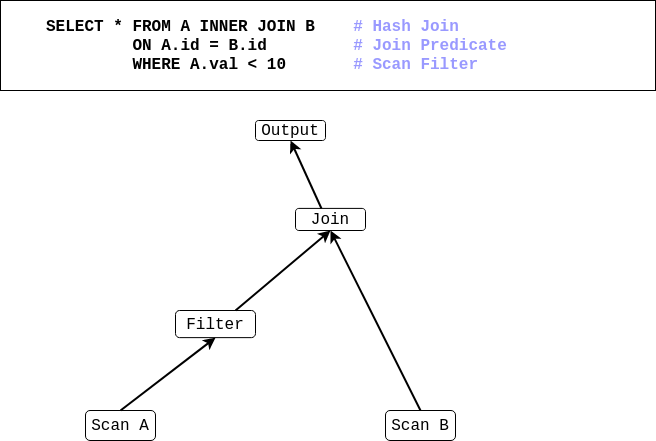
\includegraphics[scale=0.5]{images/SampleQuery.png}
    \caption{\textbf{Sample SQL Query and Plan.}}
    \label{fig:intro_query}
\end{figure}


The traditional execution technique used in most DBMSs \cite{mysql, posrgres}, the Iterator Model \cite{volcano}, became ill-suited for modern OLAP applications. It executes a query by interpreting the query plan. Each database operator implements a virtual \texttt{next()} function that returns the next tuple it can generate; each expression (i.e. addition, multiplication) also provides an virtual \texttt{evaluate()} function that takes in a tuple and returns a value. \cref{fig:volcano_graph} showcases the Iterator model with the sample query in \cref{fig:intro_query}. The operators \texttt{Scan A} and \texttt{Scan B} iterate through the table and emit the tuples to the parent operator. The filter only returns tuples that satisfy the \texttt{WHERE} clause. The join first builds a hash table, then probes it to find matches.

\begin{figure}[t!]
    \centering
    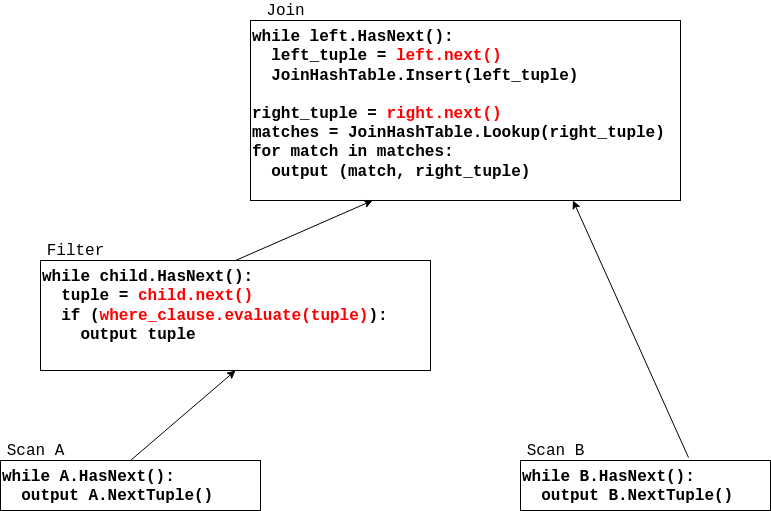
\includegraphics[scale=0.5]{images/Volcano.png}
    \caption{\textbf{The Iterator Model on the Sample SQL Query.}}
    \label{fig:volcano_graph}
\end{figure}


We can see why the Volcano model is ill-suited for in-memory DBMSs. For every tuple -- of which there can be billions in an OLAP setting -- the virtual function calls (marked in red in the figure) constitute a significant overhead.

To minimize this overhead for in-memory DBMSs, researchers have developed the Vectorization Model.



\iffalse
\section{Compilation}
\begin{figure}[H]
\centering
\begin{subfigure}{.5\textwidth}
 \centering
 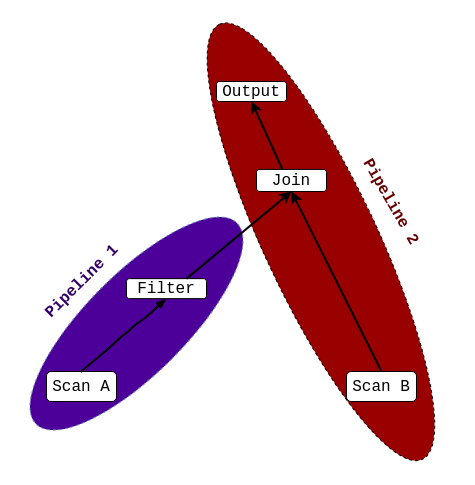
\includegraphics[width=0.9\textwidth]{images/Pipeline.png}
 \caption{Pipelines within the sample query.}
  \label{fig:pipeline_graph}
\end{subfigure}%
\begin{subfigure}{.5\textwidth}
 \centering
 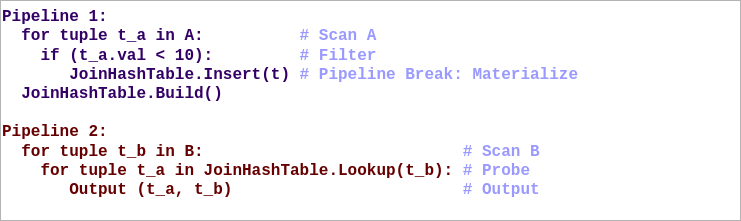
\includegraphics[width=0.9\textwidth]{images/PipelineCode.png}
 \caption{Code generated for the sample query.}
  \label{fig:pipeline_code}
\end{subfigure}
\caption{The compilation model with the sample query. Each pipeline and its corresponding code have the same color.}
\label{fig:update_map_intro}
\end{figure}


Query compilation \cite{system_r, hique, hyper_llvm} aims to eliminate the cost of interpretation by compiling the query plan down to machine code.
{
\color{red}
Describe what compilation means.
}


The data-centric compilation technique pioneered by Hyper \cite{hyper_llvm} splits the plan into several pipelines and compiles them individually. A pipeline is a sequence of relational operators that do not materialize the input result set followed by a pipeline-breaker -- an operator that does materialize the input set (e.g., to build a hash table, or to sort tuples). \cref{fig:pipeline_graph} showcases the pipelines of the sample query. The first pipeline-breaker occurs in the join operator because it needs all input tuples to build a hash table. \cref{fig:pipeline_code} lists the code generated for the query. Conceptually, it performs the same task as \cref{fig:volcano_graph} without any of the virtual function calls. In addition to eliminating interpretation, this approach maximizes register/cache efficiency because a pipeline fully processes a single tuple before fetching the next one. Compilation thus reduces both the number of instructions executed and the number cycles per instructions.
\fi

\section{Vectorization}
\begin{figure}[t!]
    \centering
    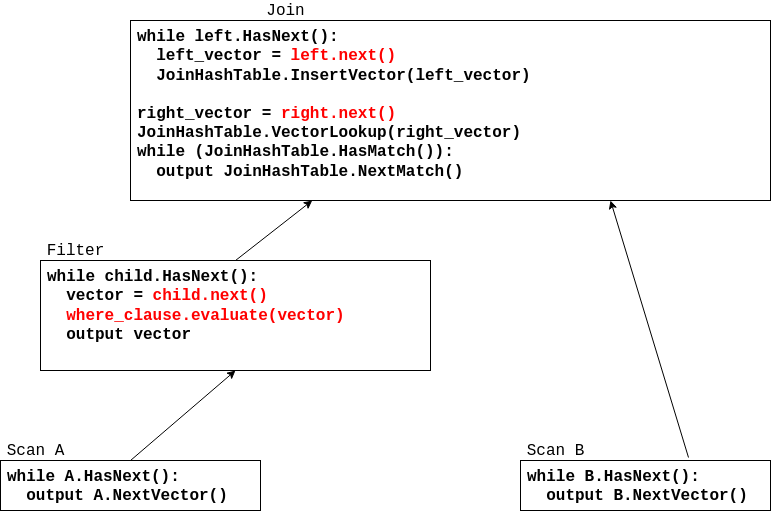
\includegraphics[scale=0.5]{images/Vectorization.png}
    \caption{\textbf{The Vectorization Model with the Sample Query} -- The code is nearly identical to that in \cref{fig:volcano_graph}}
    \label{fig:vectorization_graph}
\end{figure}

The vectorization model, pioneered by Vectorwise \cite{vectorwise}, is almost identical to the Volcano model, except that it deals with batches of tuples or \textit{vectors} (e.g., 2048 tuples at a time). The \texttt{next()} function returns a vector of tuples, and the \texttt{evaluate()} function returns a vector of values. \cref{fig:vectorization_graph} showcases vectorization model on the sample query in \cref{fig:intro_query}; it is near identical to \cref{fig:volcano_graph}.

\begin{figure}[t!]
    \centering
    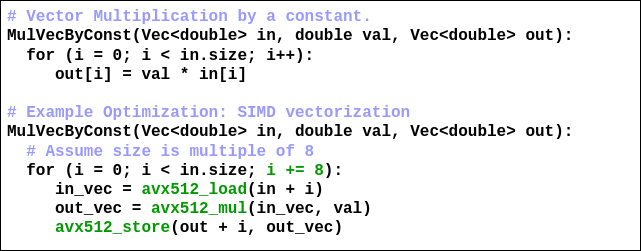
\includegraphics[scale=0.5]{images/VectorMul.png}
    \caption{\textbf{A Vectorized Multiplication Function} -- The code in green indicates compiler or programmer optimizations to exploit Intel's AVX512 features.}
    \label{fig:vector_mul}
\end{figure}
Vectorization provides two main benefits. First, it amortizes the cost of interpretation by the size of vectors. Second, most functions that operate on vectors are highly amenable to loop optimizations (e.g., loop unrolling, SIMD vectorization) by the compiler or by the programmer. Consider, for a example, the function shown in \cref{fig:vector_mul}. The iterations of the loop are independent, and the floating-point multiplication possesses a SIMD variant, which means the loop can be unrolled and vectorized by the compiler.

\iffalse
\begin{figure}[H]
    \centering
    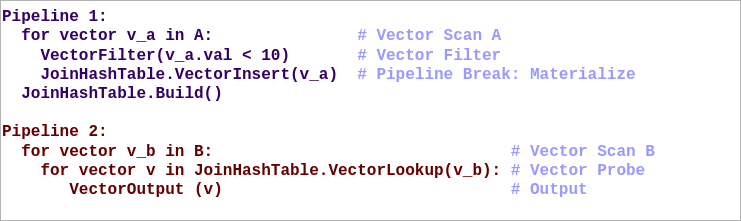
\includegraphics[scale=0.5]{images/VectorCompilation.png}
    \caption{A hybrid vectorization and compilation model with the sample query..}
    \label{fig:mix_compilation_vectorization}
\end{figure}
Our system \cite{rof, noise_page} combines both data-centric code generation and vectorization : it generates code that operates on vectors. This approach eliminates interpretation overhead and still enables loop optimizations. \cref{fig:mix_compilation_vectorization} showcases the mixed model. It differs from \cref{fig:compilation_graph} only in that it operates on vectors.
\fi


Vectorization introduces a new challenge. Individual tuples within a vector may be \textit{filtered out}, meaning that should not be processed. Only \textit{selected} tuples -- those not filtered out -- should be processed. For example, in \cref{fig:vectorization_graph}, only tuples that satisfy the \texttt{WHERE} clause should be inserted in the hash table. Next, we discuss the methods used to represent filters, i.e., to identify selected tuples within a vector.



\section{Filter Representation}
\cref{fig:repr_intro} displays the two common ways to represent filters: Selection Vectors (SelVecs) and Bitmaps. SelVecs index into the selected tuples; tuples without an index are implicitly filtered out. For Bitmaps, on the other hand, the set bits indicate the selected tuples; the unset bits indicated filtered out ones.
\begin{figure}[t!]
    \centering
    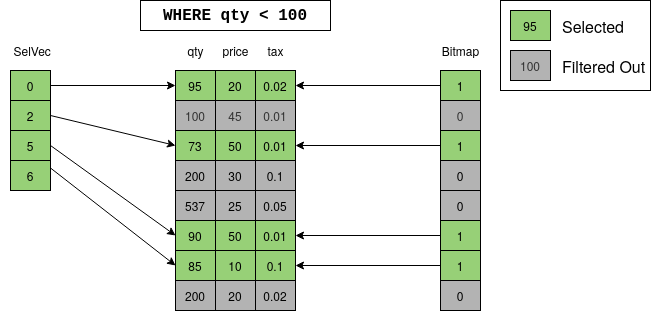
\includegraphics[scale=0.7]{images/FilterRepresentationIntro.png}
    \caption{\textbf{Filter Representation} -- Selection Vectors (left) index into the tuple vector. Bitmaps (right) are only set on selected rows.}
    \label{fig:repr_intro}
\end{figure}
Previous work has assumed one of these two representations, without providing a reason for that choice. Vectorwise \cite{vectorwise}, and work derived from it \cite{miro_adapt, everything_vectorized, sompolski_vec},  rely on SelVecs, whereas the more recent VIP \cite{orestis_bitmap} relies on Bitmaps. This paper aims to analyze the trade-offs between these two representations and derive insights for developers implementing vectorized query processing.


\chapter{Computing on Filtered Vectors}
\section{Operations on Filtered Vectors}
\begin{figure}[t!]
\centering
\begin{subfigure}{.5\textwidth}
 \centering
 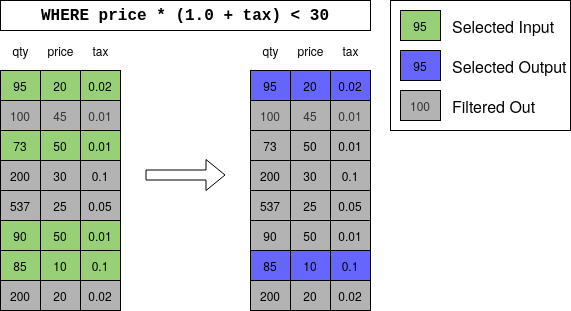
\includegraphics[width=0.9\textwidth]{images/UpdateIntro.png}
 \caption{Update operation.}
  \label{fig:update_intro}
\end{subfigure}%
\begin{subfigure}{.5\textwidth}
 \centering
 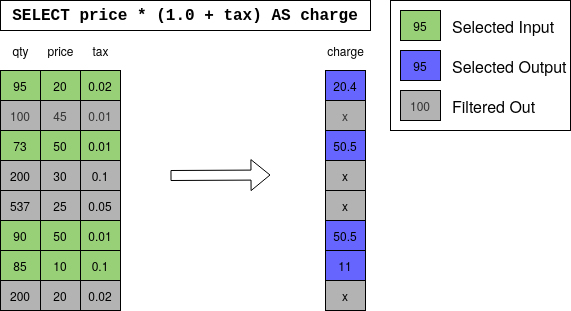
\includegraphics[width=0.9\textwidth]{images/MapIntro.png}
 \caption{Map operation.}
  \label{fig:map_intro}
\end{subfigure}
\caption{\textbf{Operations on Filtered Vectors} -- Updates change the set of selected tuple. Maps apply a function to the set of selected tuples without updating the set.}
\label{fig:update_map_intro}
\end{figure}
\cref{fig:update_map_intro} shows the two kinds of operations on vectors of tuples: Updates and Maps. Updates apply a new predicate function to the vector and update the selected tuples accordingly. A scan filter (i.e., WHERE clause) is an example of an update operation. Maps, on the other hand, keep the selected set but compute a new vector using a mapping function, or reduce the vector to a single value (e.g., for aggregation). A projection (i.e., SELECT clause) is an example of a map operation. All relational operations considered in this paper are decomposable into a set of maps and updates. \cref{fig:probe_example} shows the example of join probes. First, we compute the hashes of the input tuples; the result is a vector of hash values (Map). Then, we perform a hash table lookup using the hashes to obtain a vector of hash table entries (Map). Due to hashing collisions, the entries may not match the input, so we need to compare the join keys to filter out inexact matches (Update). We then advance the hash table chains (Map) and repeat the comparison until entries are exhausted.

\begin{figure}[t!]
    \centering
    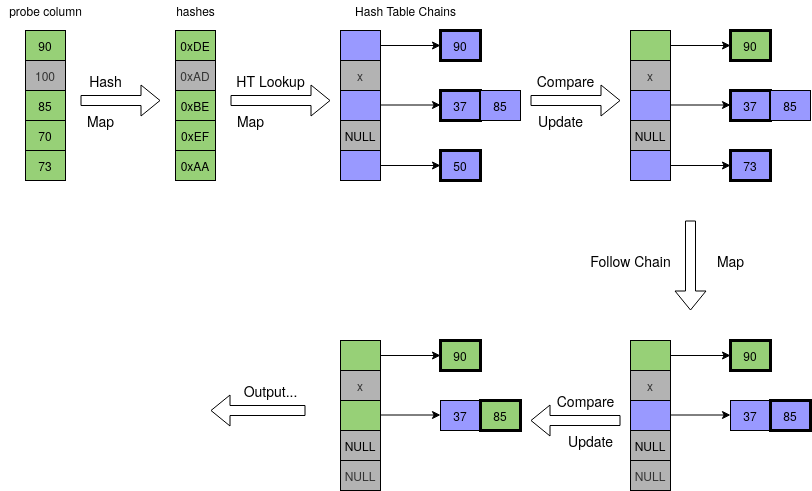
\includegraphics[scale=0.5]{images/JoinProbeExample.png}
    \caption{\textbf{Multi-step Join Probe} -- Bold squares indicate the hash table entries currently pointed to.}
    \label{fig:probe_example}
\end{figure}

Other relational operators are similarly decomposable. The next section briefly discusses transitioning between steps before we move on to the core of the thesis: optimizing each step. 

\section{Transitioning Between Steps}
In this section, we briefly talk about the cost of transitioning between steps. Most of the time, this cost is non-existent because the filter: the transition is \textit{implicit}. The hashing phase and the lookup phase in \cref{fig:probe_example} have the same selection vector. On the other hand, the Chain Following phase operates on entries that do not satisfy the comparison: the transition involves a set difference. Transitions in decomposed disjunctive filters \cite{pcq} (shown in \cref{fig:disjunctive_filter_howto}) involve both a set difference for short-circuiting and a union to get the final result.
\begin{figure}[t!]
    \centering
    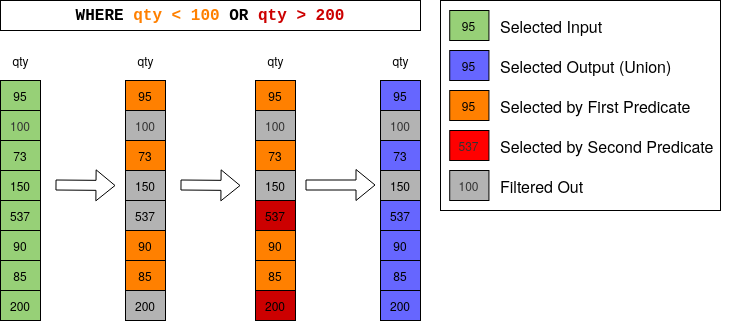
\includegraphics[scale=0.5]{images/DisjunctionHowto.png}
    \caption{\textbf{Transitioning Between Steps} -- We apply the first clause on all input tuples. In the second step, however, we only apply the second clause on those tuples that don't pass the first clause. In the third step, we take the union between the two outputs.}
    \label{fig:disjunctive_filter_howto}
\end{figure}
To the best of our knowledge, all transitions take the form of set differences (for elements that do not pass the previous predicate) and unions (to obtain the final result). These operations are cheap to implement with Bitmaps because we can easily rely on SIMD instructions. Efficiently implementing set operations on SelVecs is more complicated.  Whenever necessary, Updates can write to one additional SelVec for tuples that do not pass the filter; this second SelVec implicitly corresponds to the result of a set difference. Note that it does not overlap with the first SelVec, so a union of any of their subsets is just an array append, a fast operation. \cref{fig:disjunctive_filter_perf} shows that the overhead of set operations is negligible for both bitmaps and selection vectors. The rest of the paper, therefore, focuses on optimizing the individual steps.

\begin{figure}[t!]
    \centering
    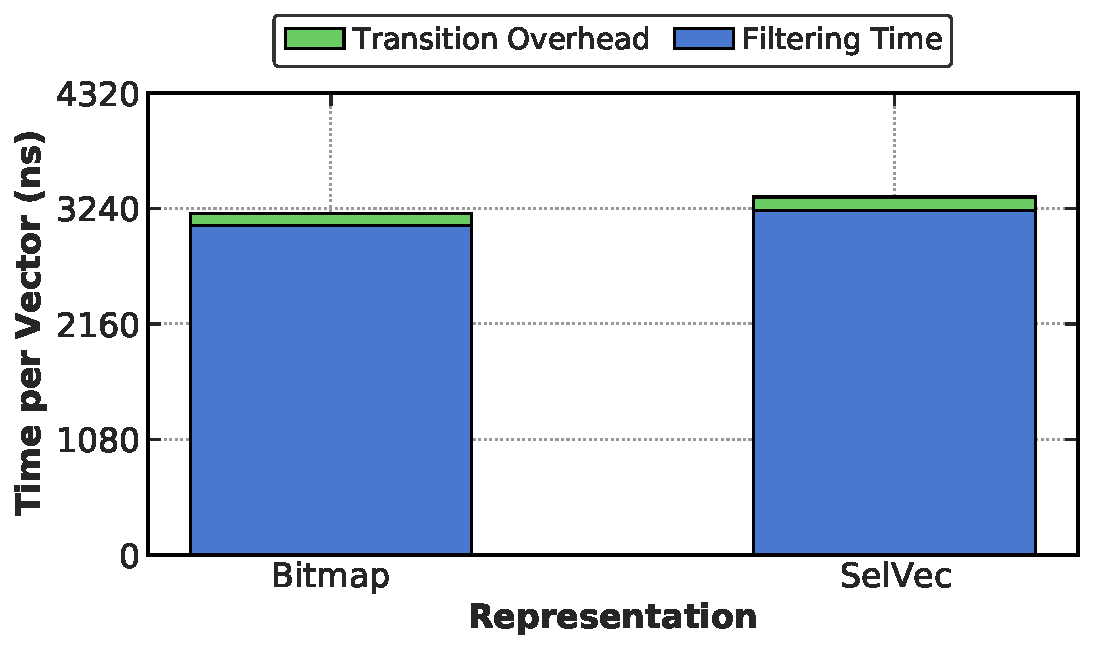
\includegraphics[scale=0.5]{eval/transition.pdf}
    \caption{\textbf{Transition Overheads} -- The overheads are $3.55\%$ and $4.06\%$ for Bitmaps and SelVecs respectively.}
    \label{fig:disjunctive_filter_perf}
\end{figure}



\section{Compute Strategies}
\begin{figure}[t!]
    \centering
    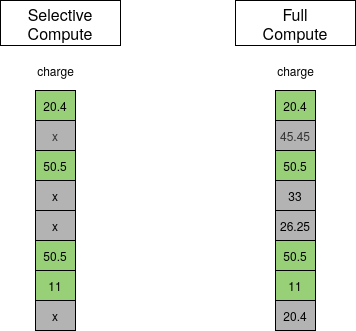
\includegraphics[scale=0.5]{images/ComputeIntro.png}
    \caption{\textbf{Compute Strategies} -- Selective Compute (left) only considers selected tuples. An \texttt{x} indicates an uninitialized value. Full Compute (right) considers all tuples.}
    \label{fig:compute_intro}
\end{figure}
 A compute strategy determines how to perform the Update or Map operations. We consider three compute strategies: Selective, Full, and Mixed Compute. As their names indicate, Selective Compute only applies the given functions to selected tuples, whereas Full Compute applies them to all tuples. \cref{fig:compute_intro} shows each approach's effect. While Full Compute usually performs more work, it greatly benefits from SIMD vectorization, simple loop structure (for loop unrolling and interleaving), and easy branch prediction. To exploit this trade-off, the third strategy, namely Mixed Strategy, switches from Full Compute to Selective Compute when the selectivity (i.e., the ratio of selected tuples) goes below a certain threshold. The next sections will show how to obtain this threshold.
 
Note that for Update operations, Full Compute is not nicely compatible with SelVecs because a slow intersection of sorted sets \cite{sorted_set} would be required to compute the final selection. This limitation will become important when choosing a strategy to implement. Furthermore, operations with side-effects (e.g., hash table build, aggregation) cannot use Full Compute for correctness reason. This thesis focuses on side-effect free operations.

Furthermore, for SelVecs, there is another dimension we did not consider: Branching Store versus Non-Branching Store. We do not focus on this dimension, for it has been studied extensively before \cite{miro_adapt}. All experiments below use the optimal branching strategy.

\section{The Filter Decision Tree}
\begin{figure}[t!]
    \centering
    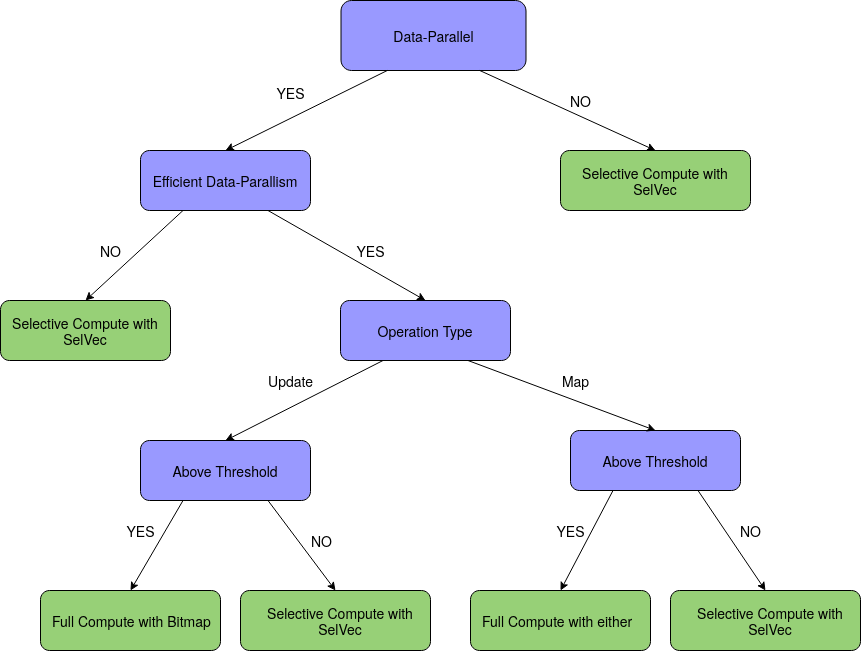
\includegraphics[scale=0.5]{images/DecisionTree.png}
    \caption{\textbf{The Filter Decision Tree.}}
    \label{fig:filter_decision_tree}
\end{figure}
\cref{fig:filter_decision_tree} shows the filter decision tree. For every kind of operation on filtered tuples, the tree indicates what the best representation and compute strategy pair is. It assumes that the developer implements all representations and compute strategies, which is a fairly costly endeavor engineering-wise. When this is not affordable, systems designers can still use this tree as a starting point before making compromises. The remaining part of this section will give a high-level rationale behind the tree. Chapter 4 will provide practical case studies that justify the shape of this tree. Chapter 5 will use the insights provided by this tree to execute an end-to-end multi-step query and show the performance gains.


\section{High Level Rationale}
\begin{figure}[t!]
\centering
\hspace*{\fill}%
\begin{subfigure}{.8\textwidth}
 \centering
 \includegraphics[width=0.9\textwidth]{images/RationaleFull.png}
 \caption{Full Compute.}
  \label{fig:rationale_full}
\end{subfigure}%
\hspace*{\fill}%
\vspace*{8pt}%

\hspace*{\fill}%  
\begin{subfigure}{.8\textwidth}
 \centering
 \includegraphics[width=0.9\textwidth]{images/RationaleBitmap.png}
 \caption{Selective Compute with a Bitmap. The iteration logic is adapted from \cite{bitmap_iteration}. The SIMD version is equivalent to Full Compute.}
  \label{fig:rationale_bitmap}
\end{subfigure}%
\hspace*{\fill}%
\vspace*{8pt}%

\hspace*{\fill}%  
\begin{subfigure}{.8\textwidth}
 \centering
 \includegraphics[width=0.9\textwidth]{images/RationaleSelVec.png}
 \caption{Selective Compute with a SelVec. The last \texttt{scatter} is only necessary to maintain consistent indices between the input and output vector during multi-step Map operations. It should otherwise be avoided due to its slowness.}
  \label{fig:rationale_selvec}
\end{subfigure}
\hspace*{\fill}%
\vspace*{8pt}%

\caption{\textbf{Implementing Vector Primitives} -- The code in green indicates the core operation (multiplication). The code in red indicates iteration logic.}
\label{fig:rationale_code}
\end{figure}


Every operation on filtered tuples is a loop, the body of which performs the actual computation. Three factors influence this loop's performance: the iteration logic, number of processed tuples, and time per processed tuple. \cref{fig:rationale_code} shows the three ways to multiply a filtered vector by a constant (a Map operation). Full Compute (e.g., \cref{fig:rationale_full}), regardless of representation, has the cheapest iteration logic because it does not need to differentiate selected indices. For Selective Compute, iterating over a Bitmap (e.g., \cref{fig:rationale_bitmap}) is more expansive than iterating over a SelVec (e.g., \cref{fig:rationale_selvec}) because of the bit operations required. On the other hand, Full Compute processes more tuples than Selective Compute, especially when the selectivity is low. Finally, SIMD instructions usually reduce the number of iterations and the number of cycles per processed tuples. SIMD code is cheapest with Full Compute; Selective Compute requires \texttt{gather} and possibly \texttt{scatter} to differentiate selected tuples.

We can use these these three factors to explain the shape of the decision tree.


\textbf{The root node}: The root of the tree addresses the case of operations on variable-length data, as is often the case for string operations (e.g., string comparison, sub-string). The number of cycles dedicated to each tuple usually far dominates the total cost. In this scenario, Full Compute is highly inefficient because it processes more tuples than Selective Compute. Also, the cost iteration logic is negligible, making representation irrelevant. We, therefore, choose to use Selective Compute, with either SelVecs or Bitmaps.


\textbf{The branching node}: We then move on to the Branching node, which addresses operations with branches in them (e.g., logical operations, \texttt{CASE} statements, \texttt{IN} statements). Branching increases the cost of SIMD relative to SISD: SISD skips unnecessary instructions, SIMD executes all of them using bit-masks. Furthermore, branches within a loop complicate loop optimizations (e.g., unrolling, interleaving). As a result, Selective Compute beats Full Compute. SelVecs only win over Bitmaps because of the simplicity of their iteration logic.

\textbf{The non-simdable node}: We now consider the non-simdable node. The most (only?) relevant operations that qualify are integer division and modulo. Complex pointer manipulations, while technically simdable using expensive scatters and gathers, also fall under this category. No compiler will auto-vectorize them, and few programmers will write and maintain such SIMD code. Like with variable-length instructions, Full Compute would introduce too much extra computation, and the representation does not matter.

\textbf{The SNBS nodes}: The most interesting nodes of this tree are those dedicated to scalar non-branching simdable (SNBS) operations; all three factors simultaneously play an essential role. Besides, for Updates, Full Compute is incompatible with SelVecs; it may be necessary to switch both compute strategy and filter representation depending on the task. The next section will justify the claims in these nodes and provide an efficient way to switch compute strategy and representation.



\chapter{Experimental Evaluation}
In this section, we experimentally justify the shape of the tree. In doing so, we will also provide a general technique that systems can use optimally switch between strategies. \cref{tab:strategies} summarizes all the strategies we implemented. We run all experiments on an Intel Xeon Platinum 8124M CPU @ 3.00GHz with AVX512 support.

\begin{table}[t!]
\centering
\begin{tabular}{|l|l|l|l|l|}
\hline
\textbf{Strategy Name} & \textbf{Representation} & \textbf{Compute} & \textbf{SIMD}      & \textbf{Compatibility} \\ \hline
SelVecPartial         & Selection Vectors       & Selective        & None               & Update and Map         \\ \hline
SelVecManual          & Selection Vectors       & Selective        & Manually Written   & Update and Map         \\ \hline
BitmapPartial         & Bitmaps                 & Selective        & None               & Update and Map         \\ \hline
BitmapFull            & Bitmaps                 & Full             & Auto Vectorization & Update and Map         \\ \hline
BitmapFullManual      & Bitmaps                 & Full             & Manually Written   & Update and Map         \\ \hline
Full                  & Either                  & Full             & Auto Vectorization & Map                    \\ \hline
FullManual            & Either                  & Full             & Manully Written    & Map                    \\ \hline
\end{tabular}
\caption{\textbf{Implemented Strategies} -- For the SIMD columns, `Auto Vectorization' indicates that we rely on compiler auto vectorization, whereas `Manually written' indicates that we write SIMD code ourselves using intrinsics. On the compatibility column, Update operations cannot use both Full Compute and Selection Vectors, which explains the last two entries.}
\label{tab:strategies}
\end{table}

\section{Variable Length Data}
\begin{figure}[t!]
\captionsetup[subfigure]{justification=justified}
\centering
\begin{subfigure}[t]{.49\linewidth}
 \centering
 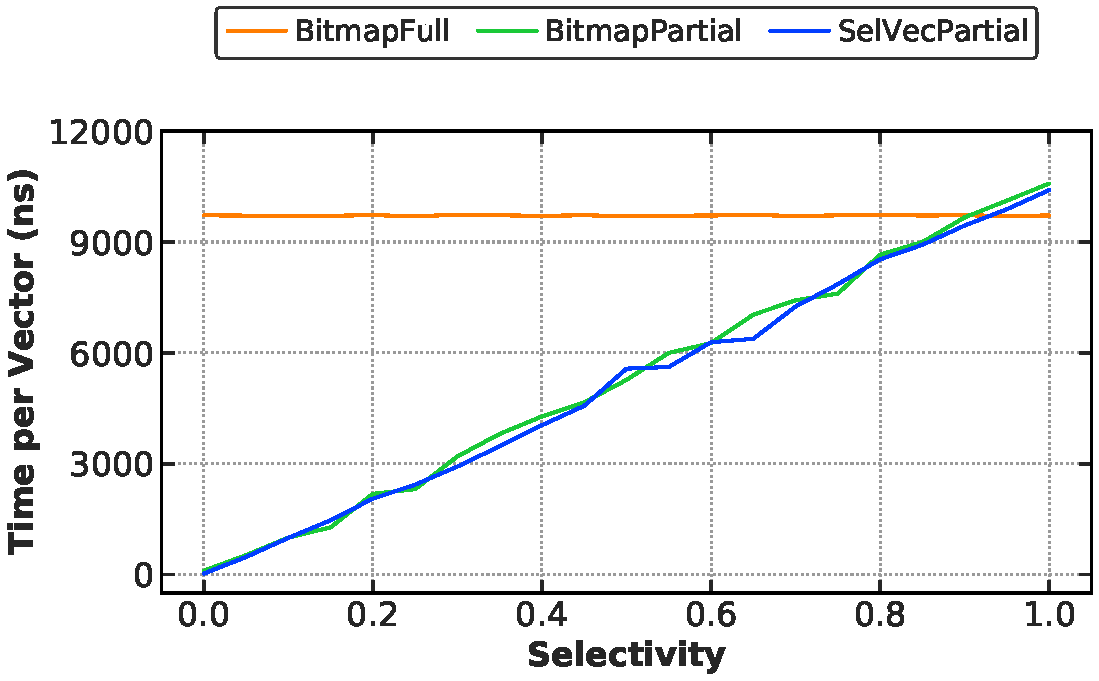
\includegraphics[width=0.9\linewidth]{eval/simple_string_update.pdf}
 \caption{Update operation corresponding to \\ \texttt{\footnotesize WHERE country < `Japan'}}
  \label{fig:varlen_update}
\end{subfigure}
\begin{subfigure}[t]{.49\linewidth}
 \centering
 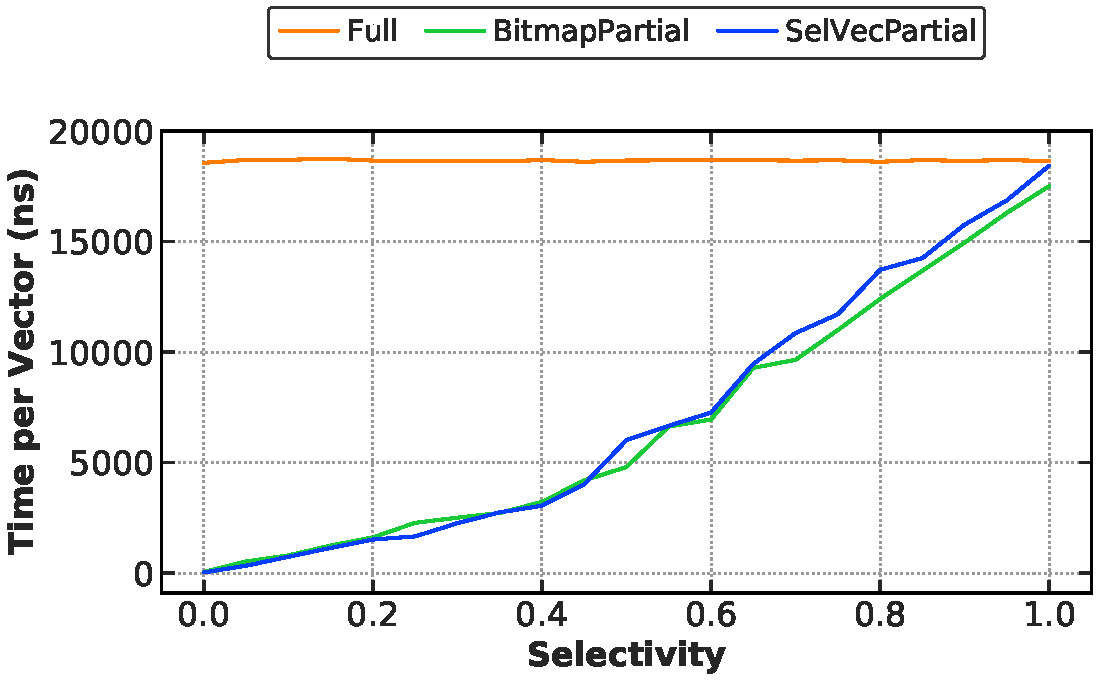
\includegraphics[width=0.9\linewidth]{eval/simple_string_map.pdf}
 \caption{Map operation corresponding to \\ \texttt{\footnotesize SELECT POSITION(`a' in country)}.}
  \label{fig:varlen_map}
\end{subfigure}
\caption{\textbf{Variable Length Data} -- Country names are all short strings that highlight the fact that even cheap variable-length operations should avoid full compute.}
\label{fig:varlen_map_update}
\end{figure}

In this section, we analyze the performance profile of operations on variable-length data. We choose cheap Update and Map operations -- string comparison, and character location on short strings (country names) -- to show that time spent per tuple typically dominates the cost of string operations. Here, the primitives process one tuple at a time; it is impossible to use SIMD registers on a vector with variable-length data.

The profiles are shown in \cref{fig:varlen_map_update}. The results confirm the high-level intuition described in the previous section. The string operations themselves are so expensive that representation matters little, and full compute is not viable. As a result, we decide to use that Selective Compute with either representation.

\section{Branching Operations}
\begin{figure}[t!]
\centering
\begin{subfigure}[t]{.49\linewidth}
 \centering
 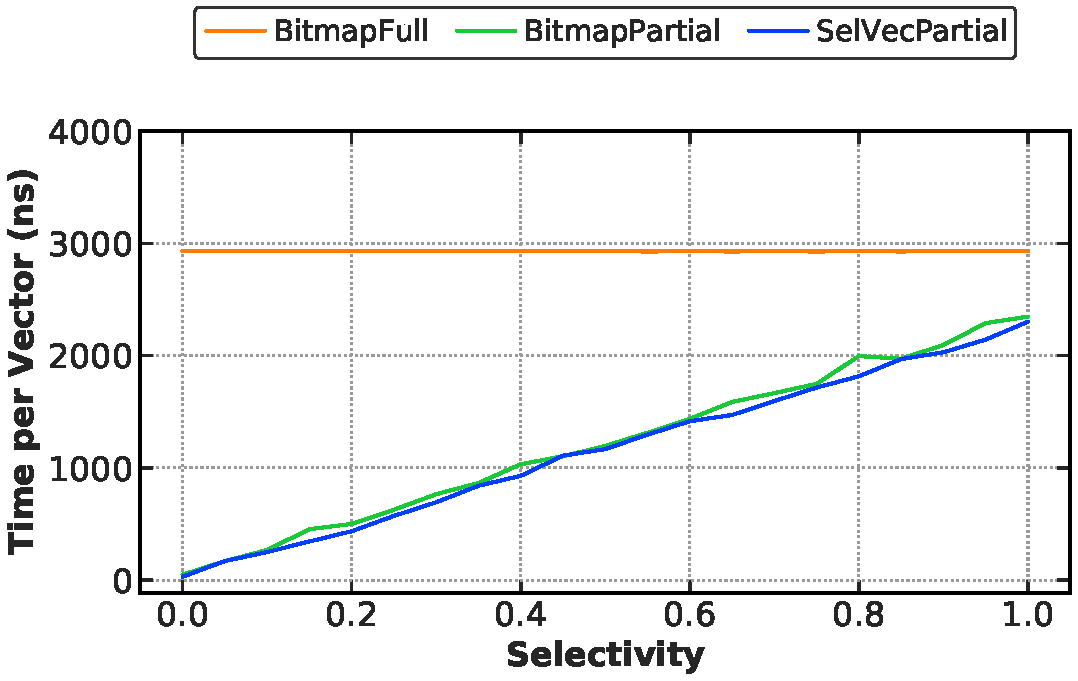
\includegraphics[width=0.9\linewidth]{eval/logical_and_update.pdf}
 \caption{Update operation corresponding to \\ \texttt{\footnotesize WHERE col1 < val1 \&\& col2 < val2}}.
  \label{fig:logical_and_update}
\end{subfigure}%
\begin{subfigure}[t]{.49\linewidth}
 \centering
 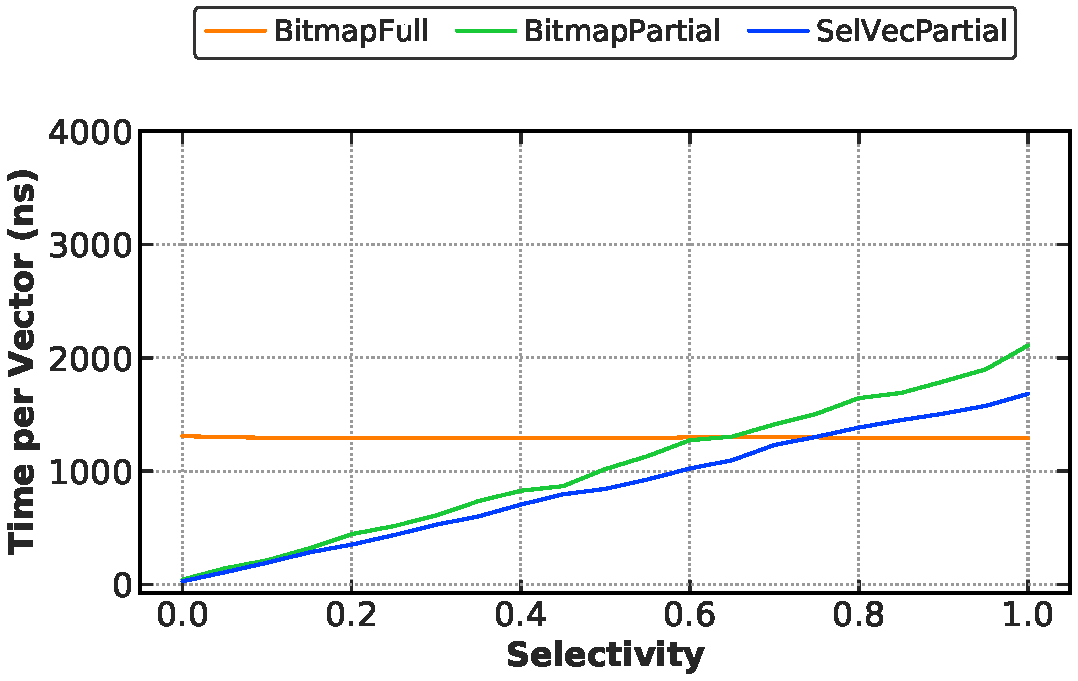
\includegraphics[width=0.9\linewidth]{eval/logical_and_map.pdf}
 \caption{Map operation corresponding to \\ \texttt{\footnotesize SELECT col1 < val1 \&\& col2 < val2}.}
  \label{fig:logical_and_map}
\end{subfigure}
\begin{subfigure}[t]{.49\linewidth}
 \centering
 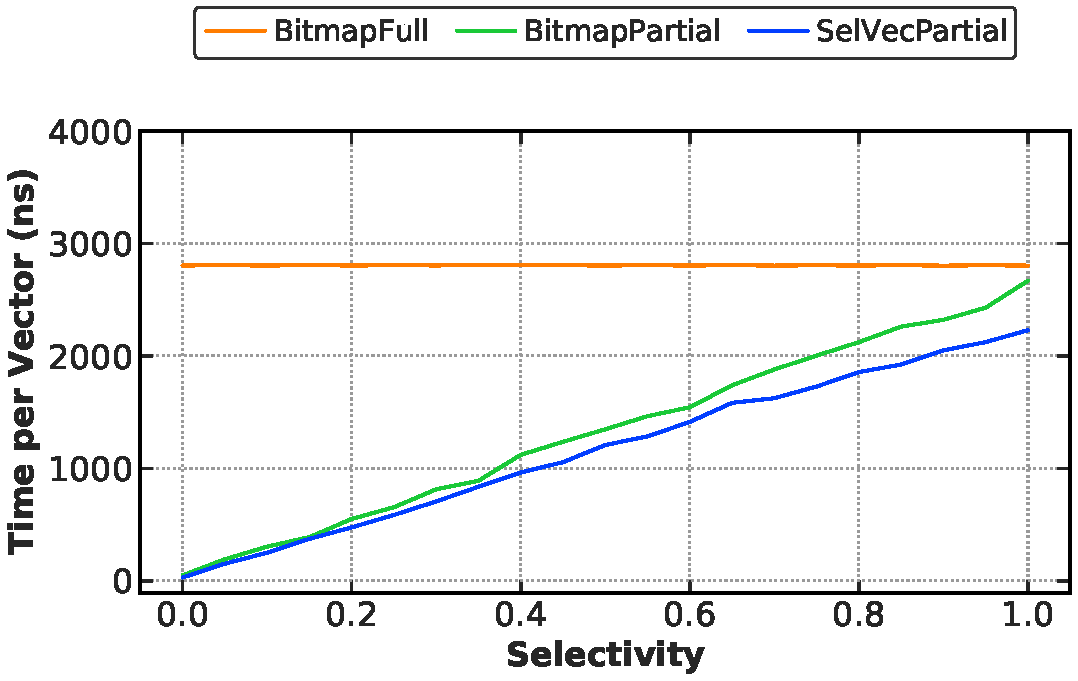
\includegraphics[width=0.9\linewidth]{eval/logical_or_update.pdf}
 \caption{Update operation corresponding to \\ \texttt{\footnotesize WHERE col1 < val1 || col2 < val2}}.
  \label{fig:logical_or_update}
\end{subfigure}%
\begin{subfigure}[t]{.49\linewidth}
 \centering
 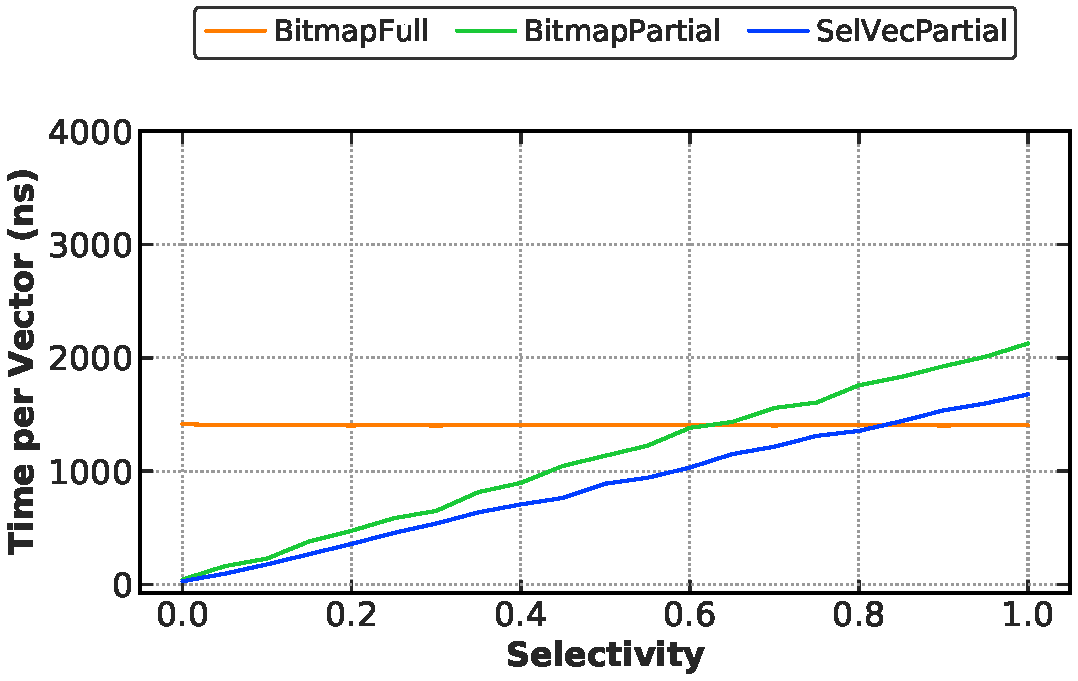
\includegraphics[width=0.9\linewidth]{eval/logical_or_map.pdf}
 \caption{Map operation corresponding to \\ \texttt{\footnotesize SELECT col1 < val1 || col2 < val2}.}
  \label{fig:logical_or_map}
\end{subfigure}

\caption{\textbf{Branching Operations} -- Each operation contains one branch because of boolean short-circuiting.}
\label{fig:logical_map_update}
\end{figure}

\begin{figure}[t!]
\centering
\begin{subfigure}[t]{.49\linewidth}
 \centering
 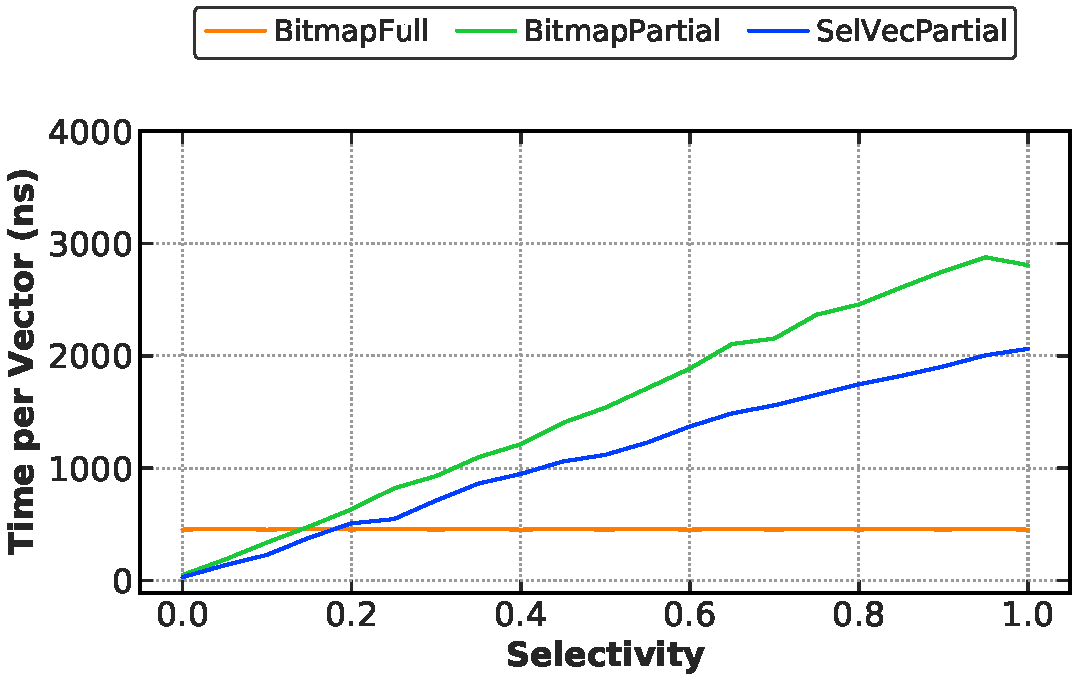
\includegraphics[width=0.9\linewidth]{eval/bitwise_and_update.pdf}
 \caption{Update operation corresponding to \\ \texttt{\footnotesize WHERE col1 < val1 \& col2 < val2}}.
  \label{fig:bitwise_and_update}
\end{subfigure}%
\begin{subfigure}[t]{.49\linewidth}
 \centering
 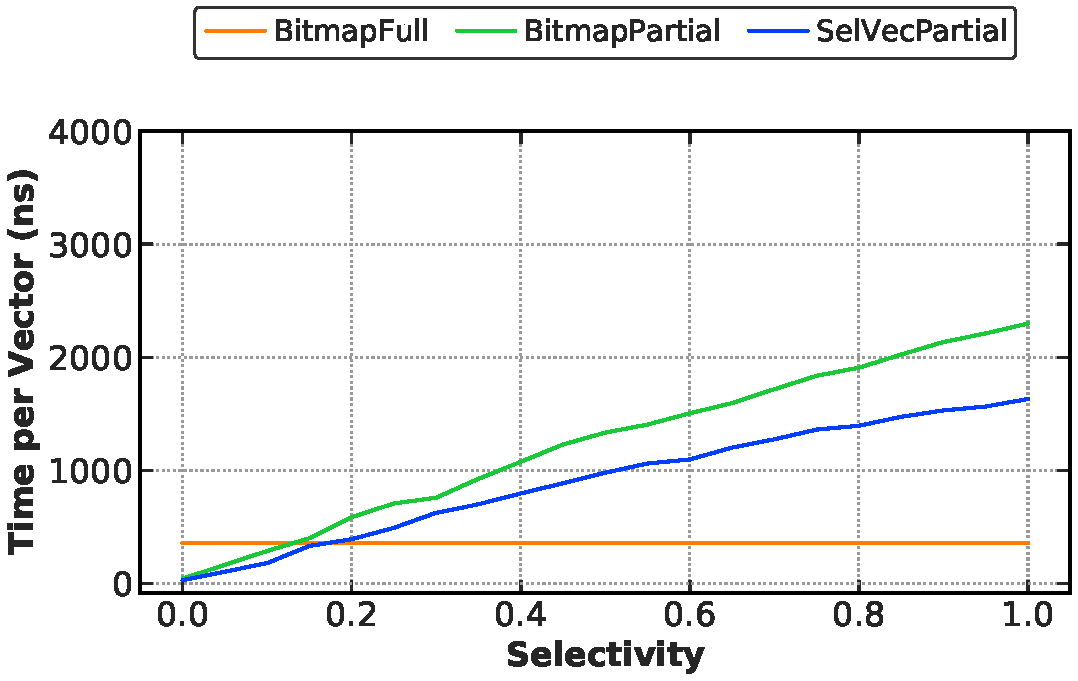
\includegraphics[width=0.9\linewidth]{eval/bitwise_and_map.pdf}
 \caption{Map operation corresponding to \\ \texttt{\footnotesize SELECT col1 < val1 \& col2 < val2}.}
  \label{fig:bitwise_and_map}
\end{subfigure}
\begin{subfigure}[t]{.49\linewidth}
 \centering
 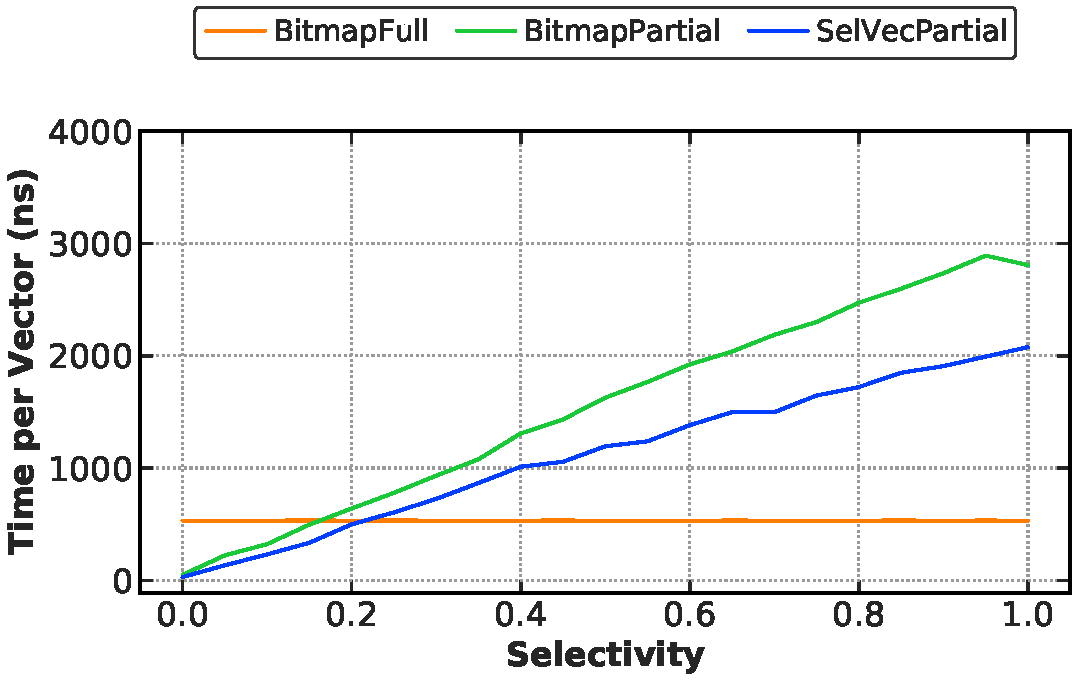
\includegraphics[width=0.9\linewidth]{eval/bitwise_or_update.pdf}
 \caption{Update operation corresponding to \\ \texttt{\footnotesize WHERE col1 < val1 | col2 < val2}}.
  \label{fig:bitwise_or_update}
\end{subfigure}%
\begin{subfigure}[t]{.49\linewidth}
 \centering
 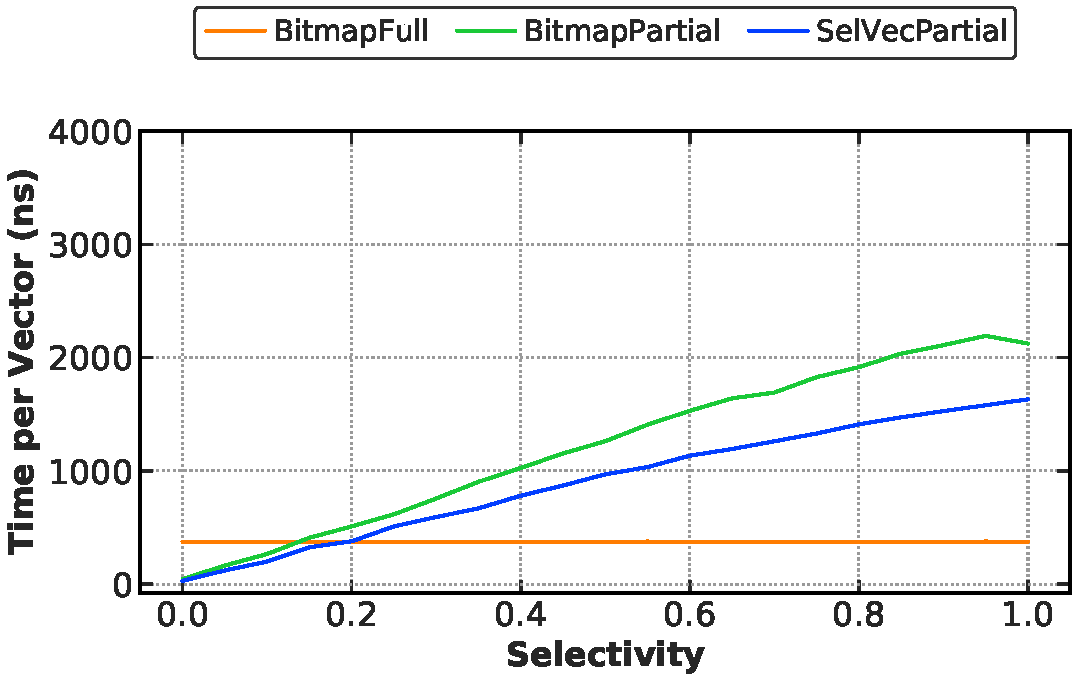
\includegraphics[width=0.9\linewidth]{eval/bitwise_or_map.pdf}
 \caption{Map operation corresponding to \\ \texttt{\footnotesize SELECT col1 < val1 | col2 < val2}.}
  \label{fig:bitwise_or_map}
\end{subfigure}

\caption{\textbf{Bitwise Operations} -- The increase in performance is due to the lack of branching.}
\label{fig:bitwise_map_update}
\end{figure}

We now consider operations involving branching execution paths. We choose the logical or/and operations because boolean short-circuiting involves a single branch to avoid evaluating unnecessary conditions. To isolate the effect of branching, we also evaluate branch-less bitwise or/and operations. We have confirmed that the compiler manages to auto-vectorize the operations.

The results for logical operations are shown in \cref{fig:logical_map_update}. We see that PartialSelVec performs better thanks to a cheaper iteration logic and that Full Compute is not viable because SIMD does not interact well with branching. \cref{fig:bitwise_map_update} confirms that branching is truly responsible for the difference in performance. The only difference between bitwise and logical operations is the short-circuiting that takes place. While Full Compute can sometimes be competitive in these scenarios (see \cref{fig:logical_or_map} at high selectivities), we decide, for the sake of simplicity, to use Selective Compute with SelVecs.


\section{Non Simdable Operations: Integer Division}
\begin{figure}[t!]
\captionsetup[subfigure]{justification=justified}
\centering
\begin{subfigure}[t]{.49\linewidth}
 \centering
 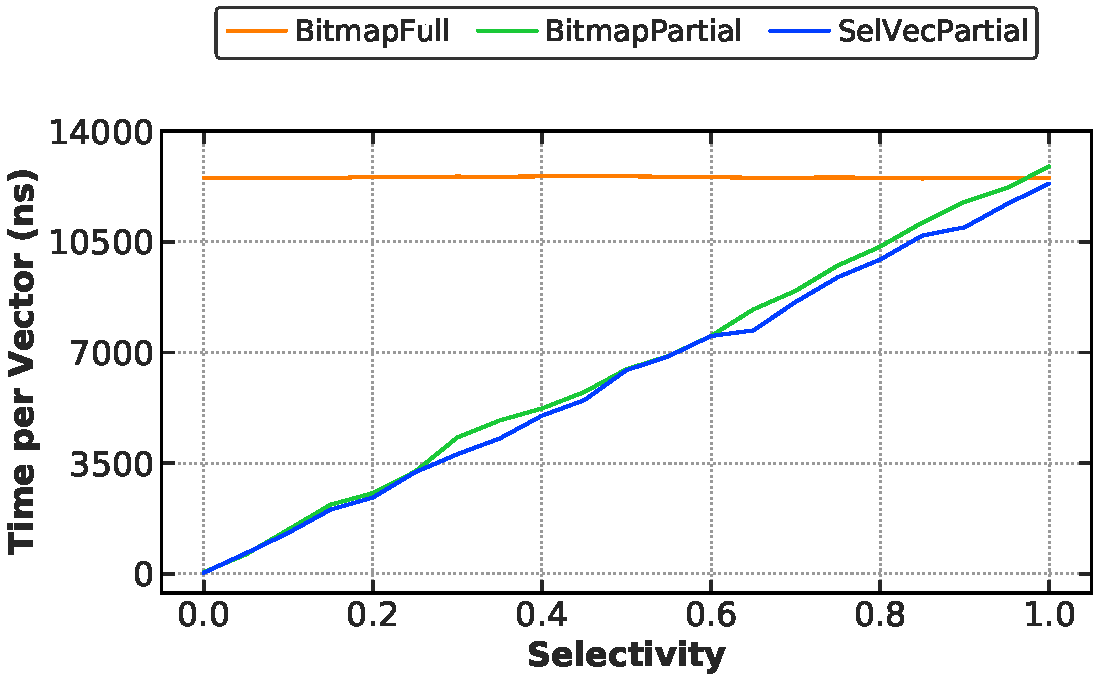
\includegraphics[width=0.9\linewidth]{eval/simple_division_update.pdf}
 \caption{Update operation corresponding to \\ \texttt{\footnotesize WHERE col1 \% col2 < val}}.
  \label{fig:division_update}
\end{subfigure}
\begin{subfigure}[t]{.49\linewidth}
 \centering
 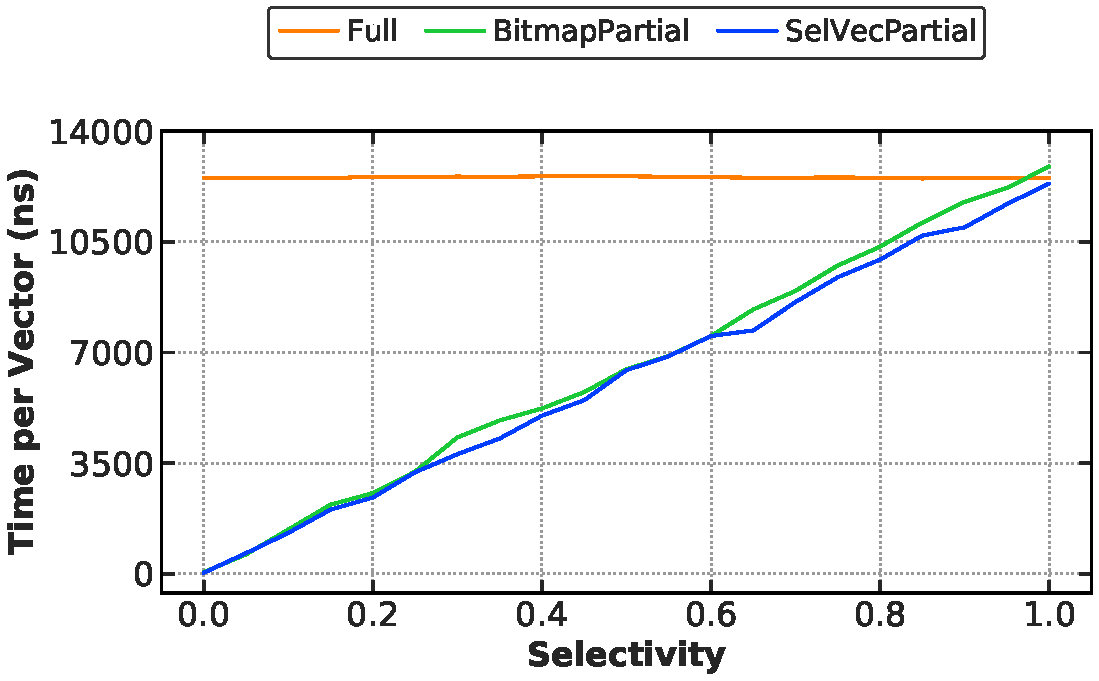
\includegraphics[width=0.9\linewidth]{eval/simple_division_map.pdf}
 \caption{Map operation corresponding to \\ \texttt{\footnotesize SELECT col1 / col2}.}
  \label{fig:division_map}
\end{subfigure}
\caption{Simple operations on a variable-length column. Country names are all short strings that highlight the fact that even cheap variable-length operations should avoid full compute.}
\label{fig:division_map_update}
\end{figure}


For this section, we consider operations involving integer division. There is no SIMD instruction for integer division; the primitives process one tuple at a time.

The results are shown in \cref{fig:division_map_update}. As predicted in the high-level rationale, the cost of integer division is so high that we recommend Selective Compute with either representation.
\section{SNBS Operations}
\label{snbs_section}
\begin{figure}[t!]
    \centering
    \makebox[\textwidth]{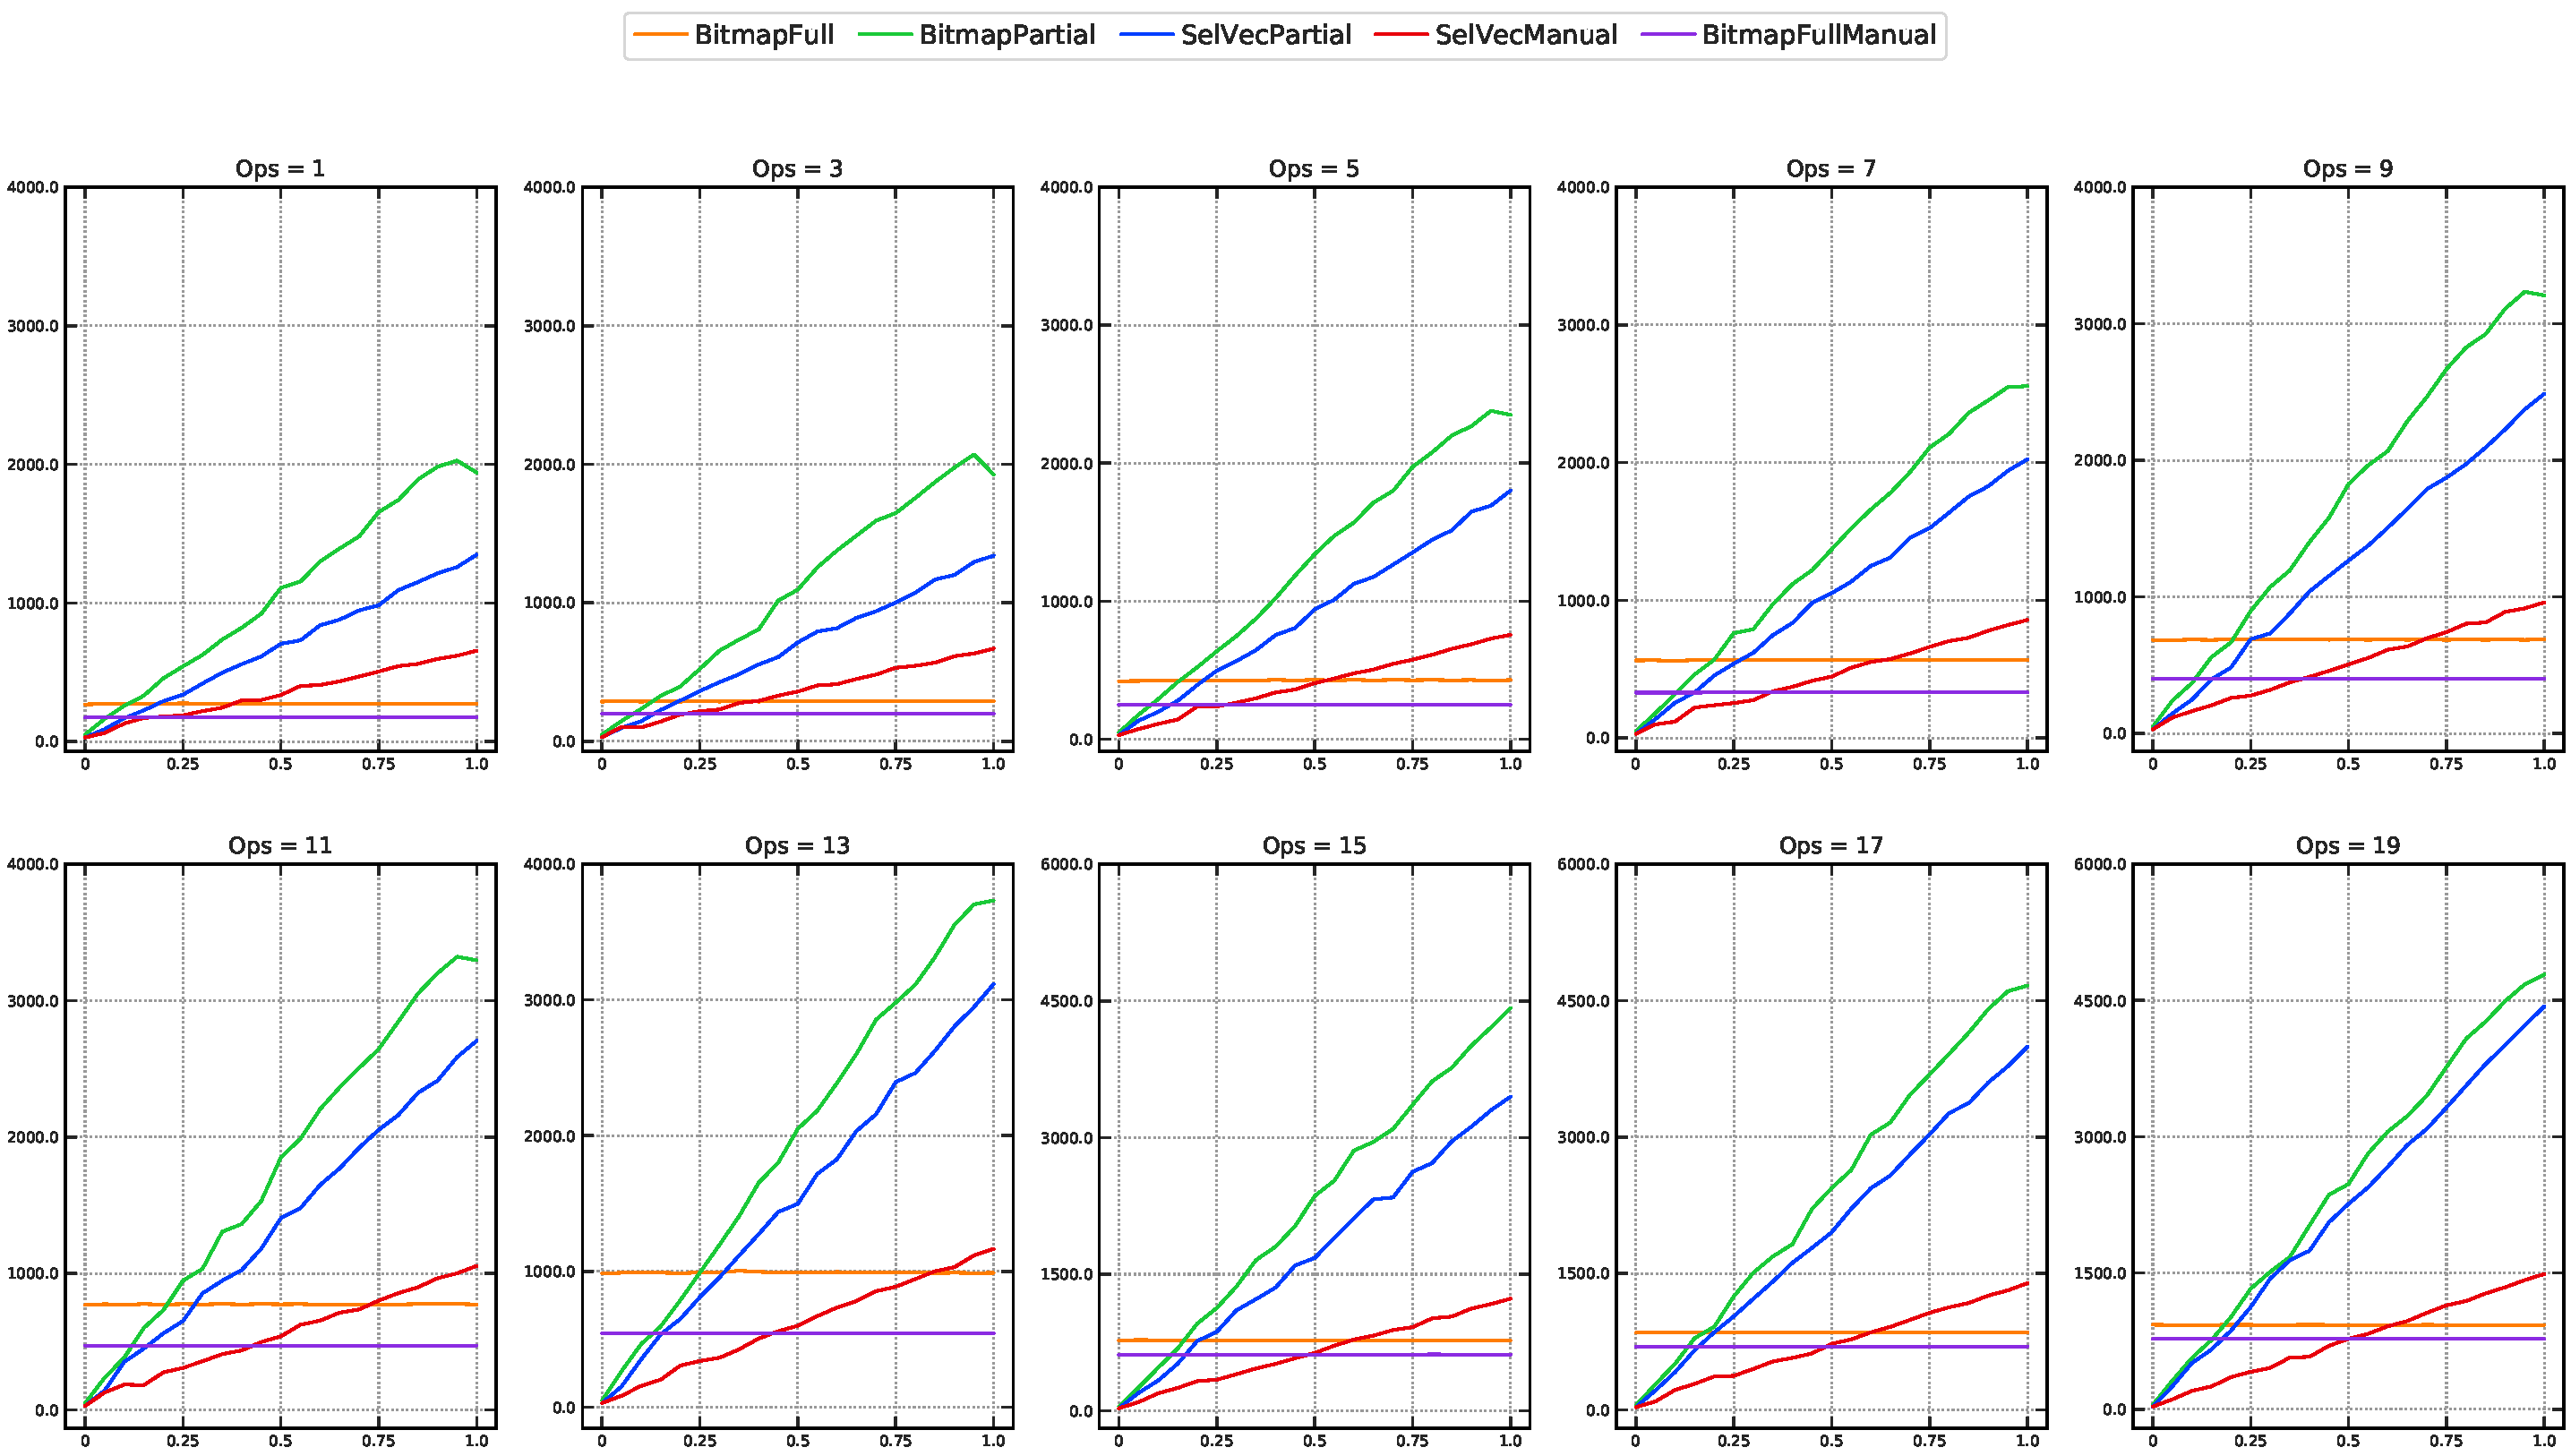
\includegraphics[width=.9\paperwidth]{eval/snbs_update.pdf}}
    \caption{\textbf{SNBS Update Operations} -- For Updates, SelVecManual relies on the \texttt{compress\_store} SIMD instruction rather than on \texttt{scatter}, which reduces its overhead.}
    \label{fig:snbs_update}
\end{figure}

\begin{figure}[t!]
    \centering
    \makebox[\textwidth]{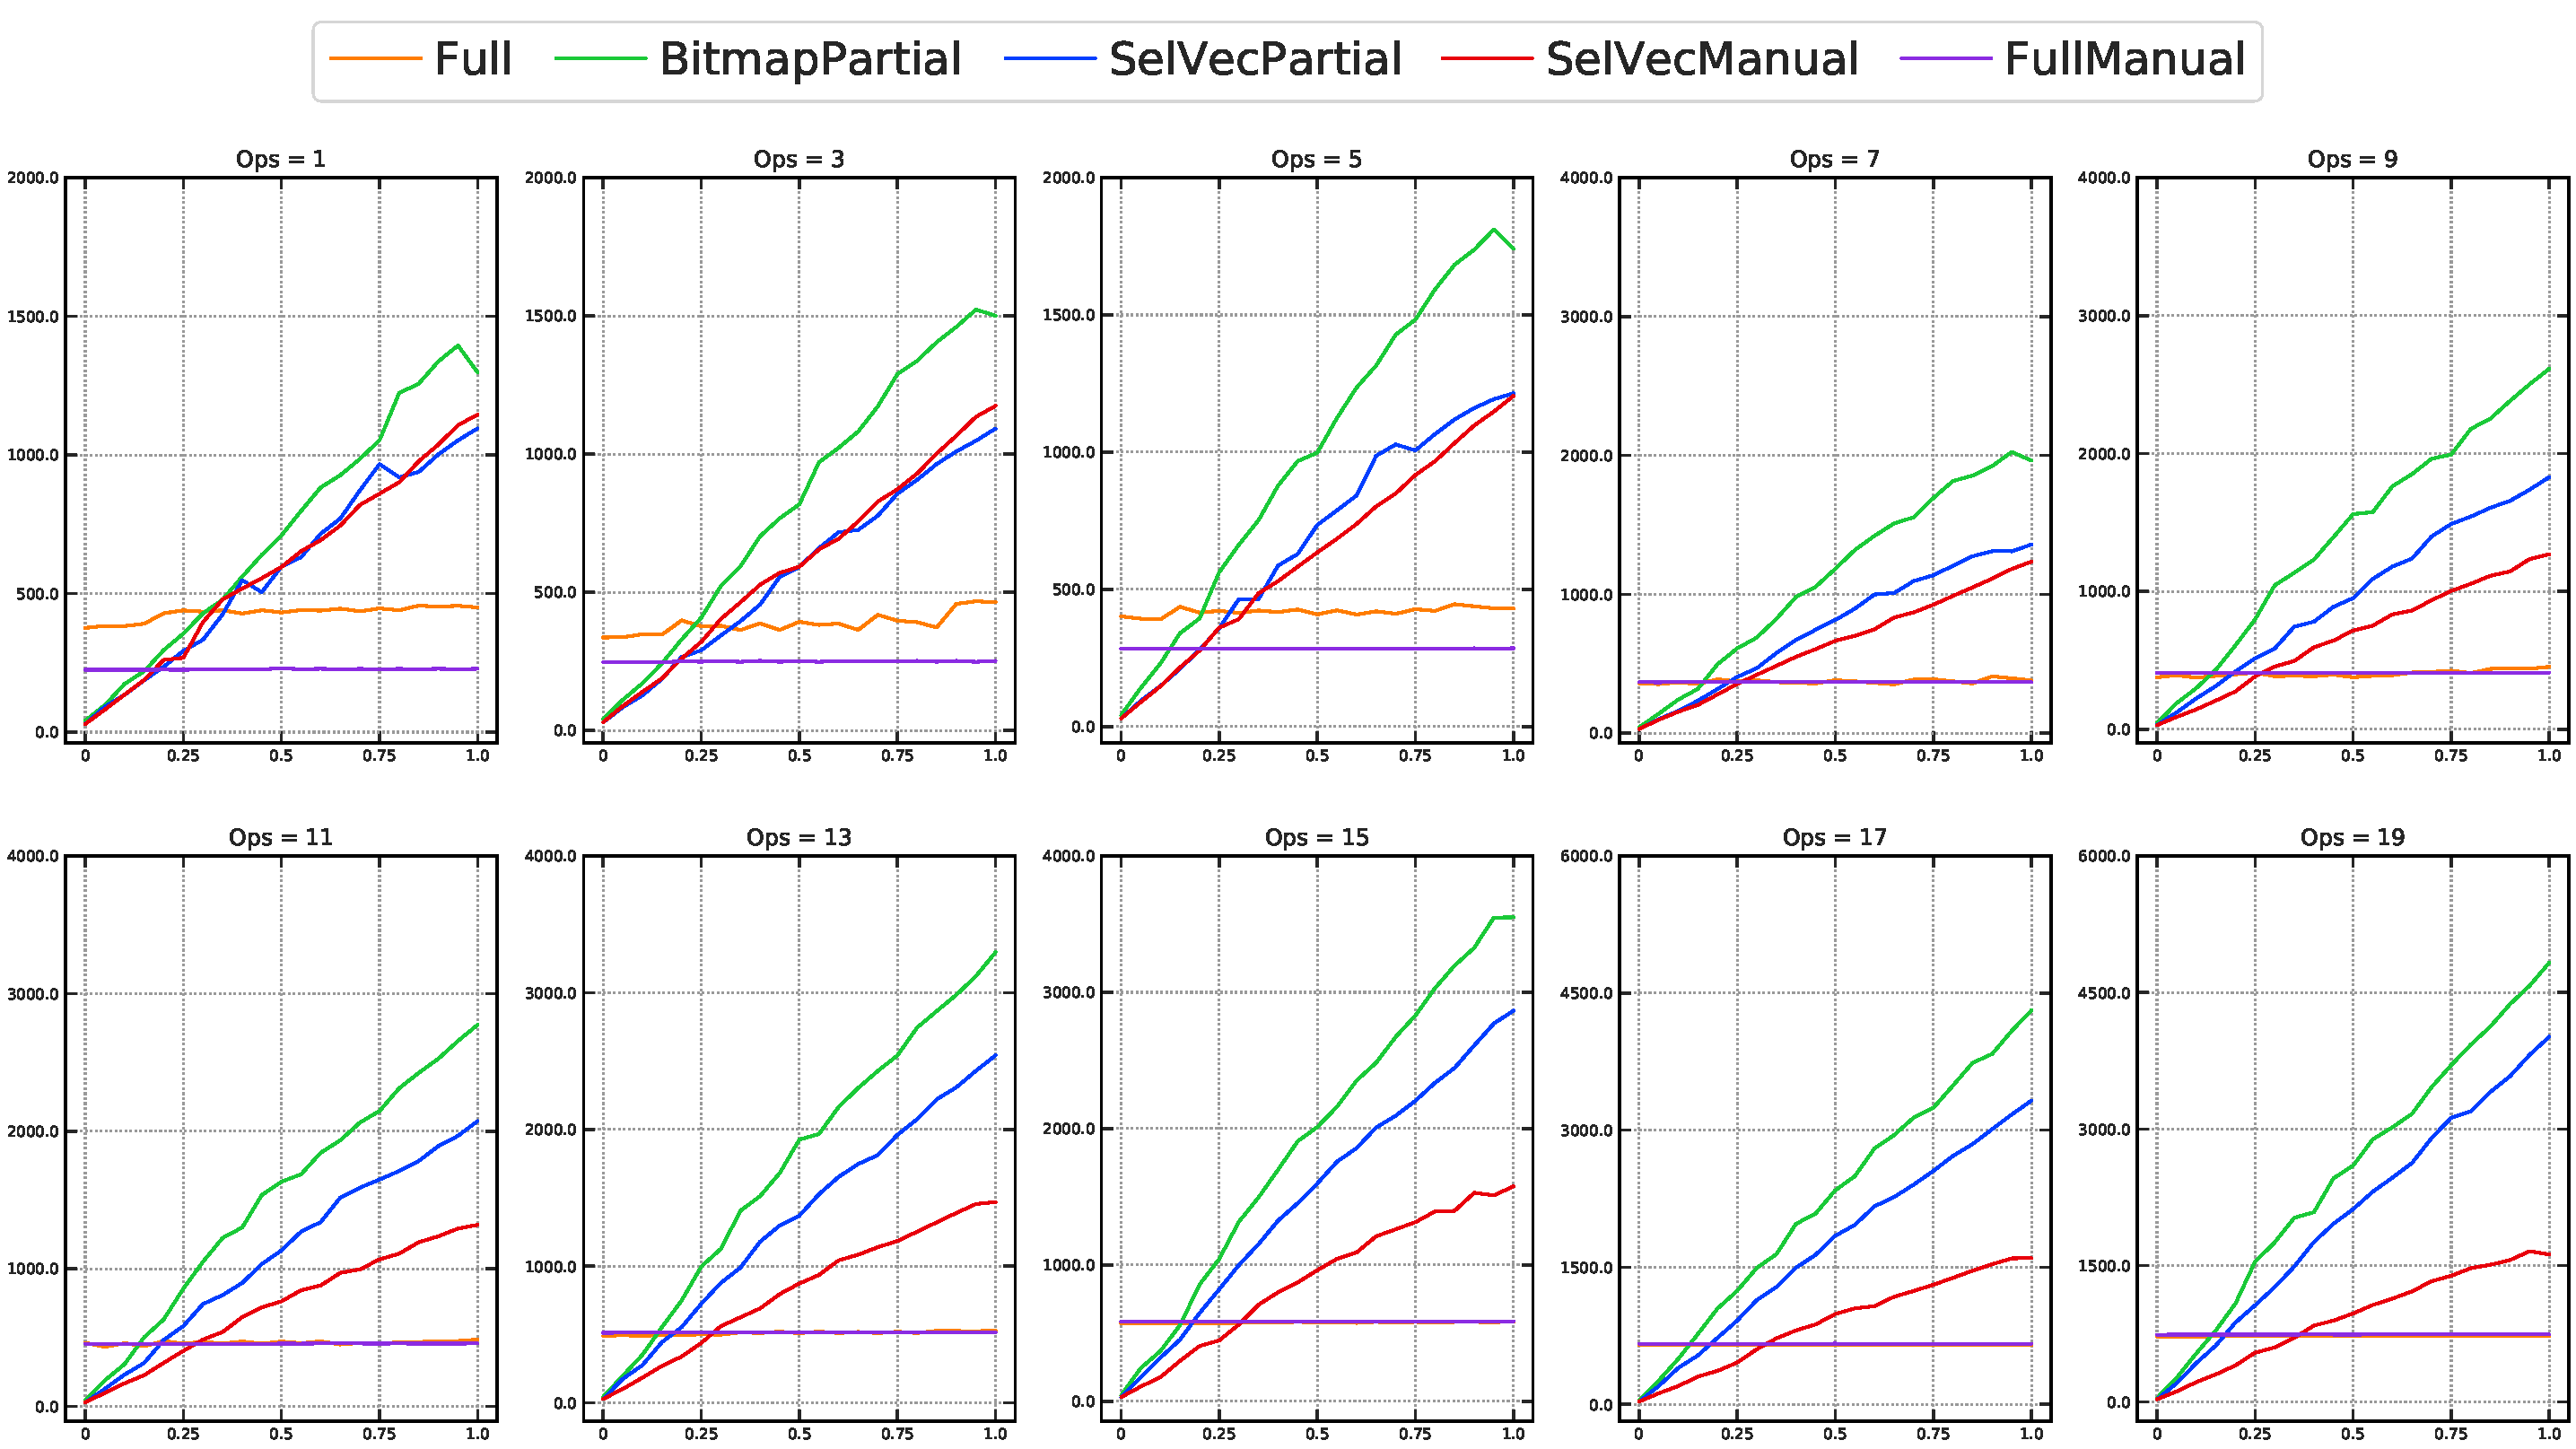
\includegraphics[width=.9\paperwidth]{eval/snbs_map.pdf}}
    \caption{\textbf{SNBS Map Operations} -- For Maps, SelVecManual relies on the \texttt{scatter} SIMD instruction, which explains why it initially does not perform better than SelVecPartial.}
    \label{fig:snbs_map}
\end{figure}



As mentioned in the rationale, the performance of SNBS operations will depend on all three performance factors: iteration logic, number of tuples processed, time per tuple. To isolate each component's effect, we experimentally evaluate the running time of Maps and Updates as a function of the selectivity and the number of single-cycle instructions (e.g., addition, subtraction, bitwise and, or, xor) in each operation.

The experimental profile of operations with multi-cycle instructions (e.g., multiplication, load, store) can be approximated by treating such operations as multiple single-cycle. The multiplying factor can be found in various instruction tables \cite{intel2019}. For example, in the machine we use for testing, a Map operation with a multiplication should have a profile similar to that of a Map operation with three additions. This method is likely not optimal, though; finding a better one is left as future work.

\cref{fig:snbs_update} and \cref{fig:snbs_map} show the performance profile of our different implementations as the number of single-cycle operations varies. The profiles correspond to what we expect based on the three performance factors, but a detailed explanation of the main features in order.
\begin{itemize}
    \item SelVecPartial generally performs better than BitmapPartial. We attribute this fact to the cost of the iteration logic. This difference is particularly relevant for cheap operations, but become irrelevant as complexity increases.
    \item Full Compute is always worst when the selectivity is low; it processes far more tuples than Selective Compute. 
    \item Full Compute is always best when the selectivity is high thanks to cheaper iteration logic and cheaper SIMD code. For example, SelVecManual always needs a gather instruction, whereas BitmapFullManual does not.
    \item SIMD beats SISD because of less time spent per tuple, as exemplified by the difference between SelVecPartial and SelVecManual.
    \item Manual Vectorization (with FullManual and BitmapFullManual) sometimes performs much better than Auto-Vectorization (with Full and BitmapFull). With further investigation of the generated code, we discovered that the compiler is overly conservative when it comes to using AVX512. AVX512 registers result in decreased CPU frequency \cite{avx512_registers}, so the compiler is careful not always to use them. It often uses AVX2 registers instead. We, on the other hand, always use AVX512.
\end{itemize}

\section{Implementing Mixed Compute}
\begin{figure}[t!]
\captionsetup[subfigure]{justification=justified}
\centering
\begin{subfigure}[t]{.49\linewidth}
 \centering
 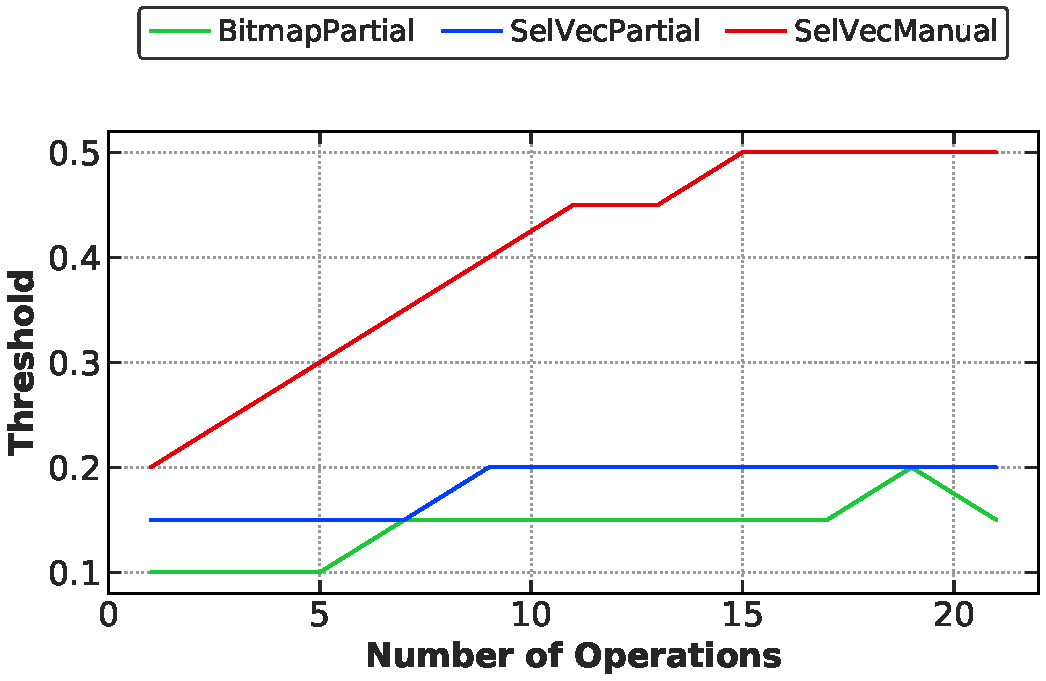
\includegraphics[width=0.9\linewidth]{eval/snbs_thres_update.pdf}
 \caption{Update thresholds between BitmapFullManual and Selective Compute strategies.}.
  \label{fig:snbs_thres_update}
\end{subfigure}
\begin{subfigure}[t]{.49\linewidth}
 \centering
 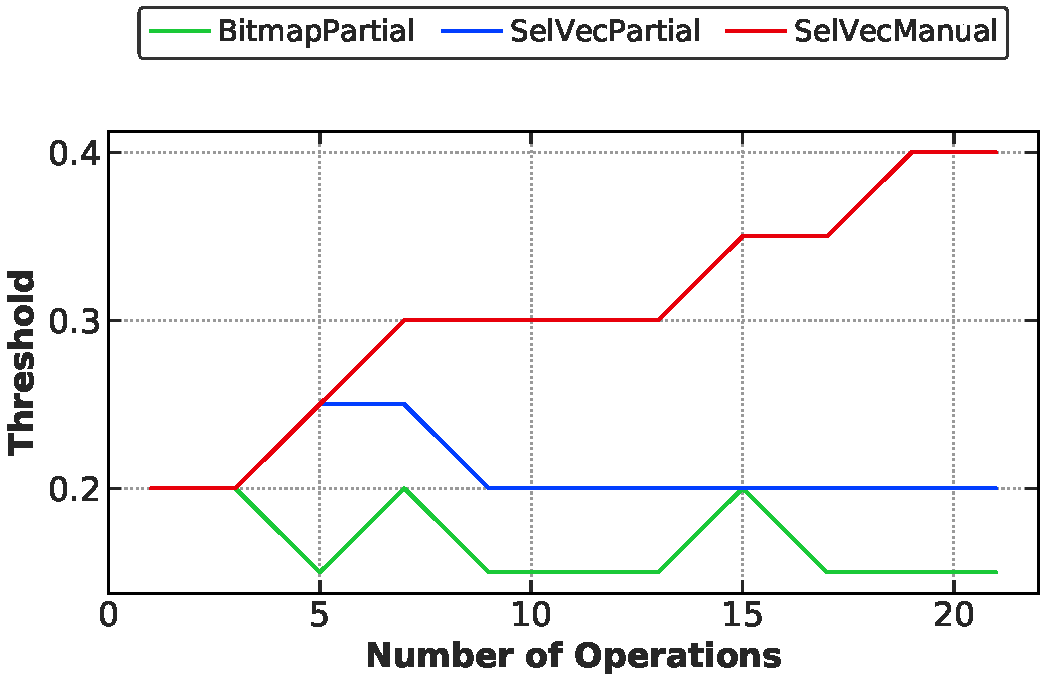
\includegraphics[width=0.9\linewidth]{eval/snbs_thres_map.pdf}
 \caption{Map thresholds between FullManual and Selective Compute strategies.}
  \label{fig:snbs_thres_map}
\end{subfigure}
\caption{\textbf{Mixed Compute Thresholds} -- The Full Compute strategies are BitmapFullManual and FullManual because compiler auto-vectorization does not consistently use AVX512 registers (as explained in the previous section).}
\label{fig:snbs_thres}
\end{figure}


Both \cref{fig:snbs_update} and \cref{fig:snbs_map} explain the necessity of Mixed Compute. Depending on the operation, there is a selectivity threshold at which we should switch from Full Compute to Selective Compute. As \cref{fig:snbs_thres} shows, this threshold a function of the cost of the operation. The curves for BitmapPartial and SelVecPartial are relatively flat because they lack the SIMD capabilities. For example, Full Compute dedicates fewer cycles per tuple even as it processes around five times more tuples at a selectivity of $0.2$. As for SelVecManual, the \texttt{gather} instruction (show in \cref{fig:rationale_selvec}) dominates its cost when the number of operations is low. As the number of operations increases, this \texttt{gather} plays a less important role in the overall performance; SelVecManual becomes more and more competitive with Full Compute because they both utilize SIMD instructions. The threshold, therefore, continually increases.

For a new query, the optimal thresholds can either be obtained by running micro-benchmarks, or by using the pre-computed thresholds in \cref{fig:snbs_thres}. The optimal strategy is as follows: 
\begin{itemize}
\item For Maps: use Full when the selectivity is above the threshold, and use SelVecManual when the selectivity is below the threshold.
\item For Update: use BitmapFull or BitmapFullManual when the selectivity is above the threshold, and use SelVecManual when the selectivity is below the threshold. There is a small cost associated with the conversion from Bitmap to SelVec, but, in practice, other operations always follow an update (e.g., there is a projection after a scan filter). The subsequent operations amortize the conversion cost.
\end{itemize}


\section{End-To-End Evaluation: TPCH Q6}
\begin{figure}[t!]
    \centering
    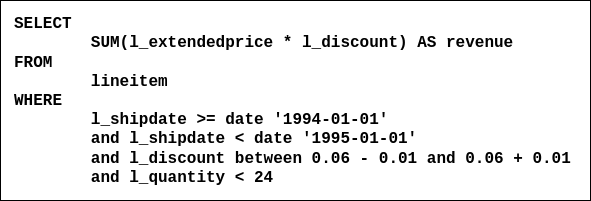
\includegraphics[scale=0.5]{images/Q6.png}
    \caption{\textbf{The TPCH Q6 query.}}
    \label{fig:tpch_q6}
\end{figure}


\begin{figure}[t!]
    \centering
    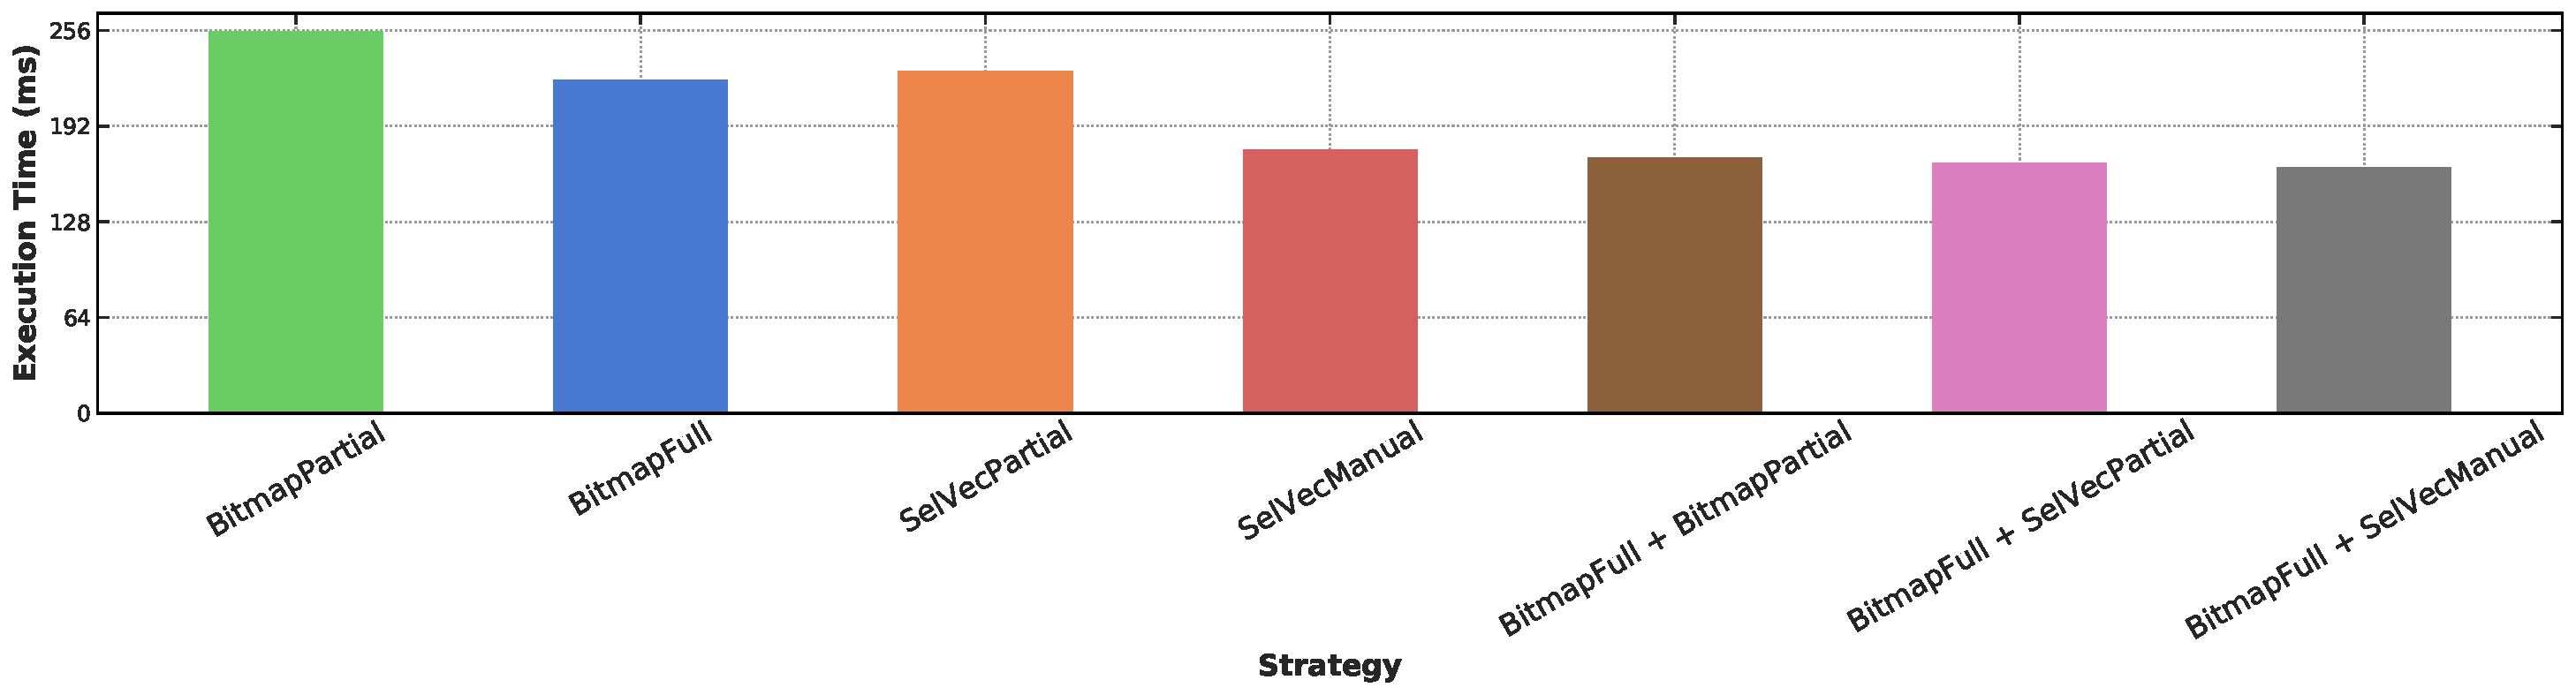
\includegraphics[width=.9\linewidth]{eval/q6_bench.pdf}
    \caption{\textbf{End-To-End Evaluation: TPCH Q6}. The scale factor is 1 (around $600000$ tuples). The horizontal line indicates the performance of the optimal strategy (BitmapFull + SelVecManual).}
    \label{fig:tpch_q6_perf}
\end{figure}


We now study the benefits of using the decision tree on a full query: TPCH Q6 \cite{tpch} (shown in \cref{fig:tpch_q6}). The query consists of five \texttt{WHERE} clause filters (Updates), and one aggregation (Map). All operations are SNBS, and all transitions are implicit. We implemented three mixed strategies: BitmapFull + BitmapPartial, BitmapFull + SelVecPartial, BitmapFull + SelVecManual. In all these strategies, the second filter triggers the threshold-based switch, which amortizes the conversion cost by a factor of four.

We compare these mixed strategies to the fixed ones of previous systems. Vectorwise and its related systems \cite{vectorwise, miro_adapt, everything_vectorized, sompolski_vec} exclusively rely on SelVecs: they cannot use on Full Compute for the five Update filters. \cite{miro_adapt} does use Full Compute on Map tasks with high selectivity, but the selectivity of Q6's final vector is in the order of $0.01$; Full Compute is too wasteful in this scenario. SelVecPartial is, therefore, representative of these systems. The recent \cite{orestis_bitmap} is more similar to BitmapFull.

The results are shown in \cref{fig:tpch_q6_perf}. As predicted in the previous chapter, BitmapFull + SelVecManual is indeed the optimal strategy.  We can also see that the fixed strategies are all worse than the mixed ones. For example, SelVecPartial is $2\times$ worse that the optimal strategy; BitmapFull is $1.37\times$ worse.

For software engineering reasons, it may be more practical to use the BitmapFull + BitmapPartial strategy. It involves only one representation (i.e., no duplicate functionality), does not require manual vectorization, and is the second-best strategy (worse by $1.2\times$). Software engineers should balance performance and maintainability.


\iffalse
\chapter{End-To-End Evaluation: TPCH Q6}


\chapter{End-To-End Evaluation: The Join Probe}
We now study the benefits of using the decision tree above on a multi-step operator involving both Maps and Updates: the join probe.

\section{Hashing}
\cref{fig:hashing} shows the cost of hashing for both strings and integers. XXHash operates on variable length data. As the root of decision tree indicates, using selective compute is the best strategy. Murmur Hash, on the other hand, is an SNBS operations. As such, Mixed Compute is the best strategy.

\section{Hash Table Lookup}
SIMD Hash table lookup can be implemented as vector gather using the hash table array as the sbase address, and the lower bits of the hash values as the indices. \cref{fig:lookup} shows the performance profile of hash table lookup. The compiler is somehow unable to perform auto-vectorization, so we only consider Manually written SIMD code. Note that the cost of a vector gather is at least 16 times that of the single-cycle instructions in the previous chapter which explains why the threshold is fairly high. Again Mixed Compute is the best strategy.

\section{Key Equality Check}
To perform SIMD equality check, we need to first gather the values that we will compare because they are part of an arbitrary hash table payload (which may contain a pointer to the next entry, other join keys and values). In addition, we need to avoid operating on null entries by using a extra SIMD mask. \cref{fig:key_check} shows that the BitmapFullManual + SelVecManual is best. We can ignore the conversion overhead because the equality check is always followed by more operations.

\section{Chain Following}
The final step we consider is chain following. The SIMD implementation, again involves a gather of the \texttt{next} pointer of hash table entries. The profile is shown in \cref{fig:chain_follow}. Unsurprisingly the Mixed Strategy described above wins again.
\fi

\chapter{Related Works}
There is a large corpus of previous work dedicated to vectorized query execution. They mostly differ from this thesis in that they do not consider the impact of filter representation in the performance of vectorized primitives. We now discuss this work and how they relate to our proposed method.
 
\cite{sompolski_vec} compares the cost of vectorization to data-centric query compilation. It combines the two approaches to generate new vectorized primitive at runtime, which is the method we use in \labelcref{snbs_section}. Using only the SelVec representation, the authors compare the performance of vectorized primitives under various compute strategies (e.g., Full v Selective Compute, Branching v Non-Branching) but do not provide a way to switch between these strategies. \cite{everything_vectorized} performs a similar analysis for whole queries rather than individual primitives.

\cite{miro_adapt} recognizes the importance of switching compute strategy at run-time. For each operation, the authors implement several \textit{flavors}, i.e., different ways to perform the same operations. They then use reinforcement learning (RL) to switch the best \textit{flavors} dynamically at run-time. This approach is more general than our static micro-benchmarks because it takes into account changes in system load. SelVec is the only representation considered, limiting the range of adaptivity on Update tasks. Besides, our decision tree provides more explainability that RL techniques. As future work, we could employ a similarly dynamic strategy to determine our thresholds.

\cite{orestis_bitmap} builds a query engine from the ground up using manually written SIMDed primitives. Its implementation of SNBS operations is most similar to our BitmapFullManual strategy. It considers a more extensive range of tasks than our side-effect-free Update/Map tasks (e.g., partitioning, building hash tables, sorting). As future work, we should perform our analysis on side-effect-full operations.
 

\chapter{Conclusion}
This work analyzed the impact of filter representation (i.e., Bitmap v SelVec) and compute strategy (i.e., Full v Selevective Compute) on the performance of vectorized primitives. We identified the factors that influence performance: iteration logic, number of tuples processed, and time spent per tuple. We explained how each combination of representation and compute strategy balances between these three strategies. Full Compute has the cheapest iteration logic, processes all tuples, but spends less time on each tuple when SIMD vectorization is possible. Full Compute is, however, only available with Bitmaps on Update tasks. Selective Compute with SelVecs has a cheaper iteration logic than Selective Compute with Bitmaps, and is more amenable to SIMD vectorization. Using these observations, we created a decision tree to help systems developers find the optimal representation for a given primitive and performed an empirical evaluation to confirm the shape of this decision tree. Finally, we showcased the benefits of our analysis using an end-to-end query involving multiple primitives.

%\appendix
%\include{appendix}

\backmatter

%\renewcommand{\baselinestretch}{1.0}\normalsize

% By default \bibsection is \chapter*, but we really want this to show
% up in the table of contents and pdf bookmarks.
\renewcommand{\bibsection}{\chapter{\bibname}}
%\renewcommand{\bibpreamble}{This text goes between the ``Bibliography''
%  header and the actual list of references}
\bibliographystyle{plainnat}
\bibliography{citations} %your bib file

\end{document}
